% Options for packages loaded elsewhere
\PassOptionsToPackage{unicode}{hyperref}
\PassOptionsToPackage{hyphens}{url}
%
\documentclass[
]{book}
\usepackage{lmodern}
\usepackage{amssymb,amsmath}
\usepackage{ifxetex,ifluatex}
\ifnum 0\ifxetex 1\fi\ifluatex 1\fi=0 % if pdftex
  \usepackage[T1]{fontenc}
  \usepackage[utf8]{inputenc}
  \usepackage{textcomp} % provide euro and other symbols
\else % if luatex or xetex
  \usepackage{unicode-math}
  \defaultfontfeatures{Scale=MatchLowercase}
  \defaultfontfeatures[\rmfamily]{Ligatures=TeX,Scale=1}
\fi
% Use upquote if available, for straight quotes in verbatim environments
\IfFileExists{upquote.sty}{\usepackage{upquote}}{}
\IfFileExists{microtype.sty}{% use microtype if available
  \usepackage[]{microtype}
  \UseMicrotypeSet[protrusion]{basicmath} % disable protrusion for tt fonts
}{}
\makeatletter
\@ifundefined{KOMAClassName}{% if non-KOMA class
  \IfFileExists{parskip.sty}{%
    \usepackage{parskip}
  }{% else
    \setlength{\parindent}{0pt}
    \setlength{\parskip}{6pt plus 2pt minus 1pt}}
}{% if KOMA class
  \KOMAoptions{parskip=half}}
\makeatother
\usepackage{xcolor}
\IfFileExists{xurl.sty}{\usepackage{xurl}}{} % add URL line breaks if available
\IfFileExists{bookmark.sty}{\usepackage{bookmark}}{\usepackage{hyperref}}
\hypersetup{
  pdftitle={연구데이터 분석과정 (R프로그래밍)},
  pdfauthor={한국생명공학연구원 김하성},
  hidelinks,
  pdfcreator={LaTeX via pandoc}}
\urlstyle{same} % disable monospaced font for URLs
\usepackage{color}
\usepackage{fancyvrb}
\newcommand{\VerbBar}{|}
\newcommand{\VERB}{\Verb[commandchars=\\\{\}]}
\DefineVerbatimEnvironment{Highlighting}{Verbatim}{commandchars=\\\{\}}
% Add ',fontsize=\small' for more characters per line
\usepackage{framed}
\definecolor{shadecolor}{RGB}{248,248,248}
\newenvironment{Shaded}{\begin{snugshade}}{\end{snugshade}}
\newcommand{\AlertTok}[1]{\textcolor[rgb]{0.94,0.16,0.16}{#1}}
\newcommand{\AnnotationTok}[1]{\textcolor[rgb]{0.56,0.35,0.01}{\textbf{\textit{#1}}}}
\newcommand{\AttributeTok}[1]{\textcolor[rgb]{0.77,0.63,0.00}{#1}}
\newcommand{\BaseNTok}[1]{\textcolor[rgb]{0.00,0.00,0.81}{#1}}
\newcommand{\BuiltInTok}[1]{#1}
\newcommand{\CharTok}[1]{\textcolor[rgb]{0.31,0.60,0.02}{#1}}
\newcommand{\CommentTok}[1]{\textcolor[rgb]{0.56,0.35,0.01}{\textit{#1}}}
\newcommand{\CommentVarTok}[1]{\textcolor[rgb]{0.56,0.35,0.01}{\textbf{\textit{#1}}}}
\newcommand{\ConstantTok}[1]{\textcolor[rgb]{0.00,0.00,0.00}{#1}}
\newcommand{\ControlFlowTok}[1]{\textcolor[rgb]{0.13,0.29,0.53}{\textbf{#1}}}
\newcommand{\DataTypeTok}[1]{\textcolor[rgb]{0.13,0.29,0.53}{#1}}
\newcommand{\DecValTok}[1]{\textcolor[rgb]{0.00,0.00,0.81}{#1}}
\newcommand{\DocumentationTok}[1]{\textcolor[rgb]{0.56,0.35,0.01}{\textbf{\textit{#1}}}}
\newcommand{\ErrorTok}[1]{\textcolor[rgb]{0.64,0.00,0.00}{\textbf{#1}}}
\newcommand{\ExtensionTok}[1]{#1}
\newcommand{\FloatTok}[1]{\textcolor[rgb]{0.00,0.00,0.81}{#1}}
\newcommand{\FunctionTok}[1]{\textcolor[rgb]{0.00,0.00,0.00}{#1}}
\newcommand{\ImportTok}[1]{#1}
\newcommand{\InformationTok}[1]{\textcolor[rgb]{0.56,0.35,0.01}{\textbf{\textit{#1}}}}
\newcommand{\KeywordTok}[1]{\textcolor[rgb]{0.13,0.29,0.53}{\textbf{#1}}}
\newcommand{\NormalTok}[1]{#1}
\newcommand{\OperatorTok}[1]{\textcolor[rgb]{0.81,0.36,0.00}{\textbf{#1}}}
\newcommand{\OtherTok}[1]{\textcolor[rgb]{0.56,0.35,0.01}{#1}}
\newcommand{\PreprocessorTok}[1]{\textcolor[rgb]{0.56,0.35,0.01}{\textit{#1}}}
\newcommand{\RegionMarkerTok}[1]{#1}
\newcommand{\SpecialCharTok}[1]{\textcolor[rgb]{0.00,0.00,0.00}{#1}}
\newcommand{\SpecialStringTok}[1]{\textcolor[rgb]{0.31,0.60,0.02}{#1}}
\newcommand{\StringTok}[1]{\textcolor[rgb]{0.31,0.60,0.02}{#1}}
\newcommand{\VariableTok}[1]{\textcolor[rgb]{0.00,0.00,0.00}{#1}}
\newcommand{\VerbatimStringTok}[1]{\textcolor[rgb]{0.31,0.60,0.02}{#1}}
\newcommand{\WarningTok}[1]{\textcolor[rgb]{0.56,0.35,0.01}{\textbf{\textit{#1}}}}
\usepackage{longtable,booktabs}
% Correct order of tables after \paragraph or \subparagraph
\usepackage{etoolbox}
\makeatletter
\patchcmd\longtable{\par}{\if@noskipsec\mbox{}\fi\par}{}{}
\makeatother
% Allow footnotes in longtable head/foot
\IfFileExists{footnotehyper.sty}{\usepackage{footnotehyper}}{\usepackage{footnote}}
\makesavenoteenv{longtable}
\usepackage{graphicx}
\makeatletter
\def\maxwidth{\ifdim\Gin@nat@width>\linewidth\linewidth\else\Gin@nat@width\fi}
\def\maxheight{\ifdim\Gin@nat@height>\textheight\textheight\else\Gin@nat@height\fi}
\makeatother
% Scale images if necessary, so that they will not overflow the page
% margins by default, and it is still possible to overwrite the defaults
% using explicit options in \includegraphics[width, height, ...]{}
\setkeys{Gin}{width=\maxwidth,height=\maxheight,keepaspectratio}
% Set default figure placement to htbp
\makeatletter
\def\fps@figure{htbp}
\makeatother
\setlength{\emergencystretch}{3em} % prevent overfull lines
\providecommand{\tightlist}{%
  \setlength{\itemsep}{0pt}\setlength{\parskip}{0pt}}
\setcounter{secnumdepth}{5}
\usepackage{booktabs}
\usepackage[]{natbib}
\bibliographystyle{apalike}

\title{연구데이터 분석과정 (R프로그래밍)}
\author{한국생명공학연구원 김하성}
\date{2020-10-12}

\begin{document}
\maketitle

{
\setcounter{tocdepth}{1}
\tableofcontents
}
\hypertarget{introduction-uxac15uxc758-uxac1cuxc694}{%
\chapter{Introduction 강의 개요}\label{introduction-uxac15uxc758-uxac1cuxc694}}

\begin{itemize}
\tightlist
\item
  장소: 코빅
\item
  강사: 한국생명공학연구원 바이오합성연구센터 김하성
\item
  연락처: 042-860-4372, \href{mailto:haseong@kribb.re.kr}{\nolinkurl{haseong@kribb.re.kr}} (생명연 연구동 1143)
\end{itemize}

\hypertarget{references-books-uxcc38uxace0-uxad50uxc81c}{%
\section{References books 참고 교제}\label{references-books-uxcc38uxace0-uxad50uxc81c}}

\begin{itemize}
\tightlist
\item
  Using R for Introductory Statistics by John Verzani

  \begin{itemize}
  \tightlist
  \item
    Free version of 1st Edition

    \begin{itemize}
    \tightlist
    \item
      \url{https://cran.r-project.org/doc/contrib/Verzani-SimpleR.pdf}
    \end{itemize}
  \item
    Second edition

    \begin{itemize}
    \tightlist
    \item
      \url{https://www.crcpress.com/Using-R-for-Introductory-Statistics-Second-Edition/Verzani/p/book/9781466590731}
    \end{itemize}
  \end{itemize}
\item
  R for Data Science (\url{https://r4ds.had.co.nz}, \url{https://github.com/hadley})
\item
  Bioinformatics Data Skills by Vince Buffalo (\url{http://2.droppdf.com/files/5aTvl/bioinformatics-data-skills.pdf})
\item
  First Course in Statistical Programming with R by Braun and
  Murdoch (\url{https://www.cambridge.org/core/books/first-course-in-statistical-programming-with-r/C9F088122AB40517B07FA77F2F0FDE2F})
\item
  Introductory Statistics with R by Dalgaard (\url{http://www.academia.dk/BiologiskAntropologi/Epidemiologi/PDF/Introductory_Statistics_with_R__2nd_ed.pdf})
\item
  Modern Applied Statistics with S by Venables and Ripley (\url{http://www.bagualu.net/wordpress/wp-content/uploads/2015/10/Modern_Applied_Statistics_With_S.pdf})
\item
  일반통계학 (영지문화사, 김우철 외)
\end{itemize}

\hypertarget{references-uxcc38uxace0-uxc790uxb8cc}{%
\section{References 참고 자료}\label{references-uxcc38uxace0-uxc790uxb8cc}}

\begin{itemize}
\tightlist
\item
  R 홈페이지 \url{https://www.r-project.org/}
\item
  Rstudio 홈페이지 \url{https://www.rstudio.com/}
\item
  Packages for biologists \url{https://www.bioconductor.org/}
\item
  R 기본 문서들 (소개, 사용, 설치, 운영) \url{https://cran.r-project.org/manuals.html}
\item
  R ebooks \url{https://bookdown.org/}
\item
  Cheat Sheets \url{https://www.rstudio.com/resources/cheatsheets/}
\item
  \url{https://resources.rstudio.com/}
\item
  \url{http://shiny.rstudio.com/tutorial/}
\end{itemize}

\hypertarget{schedule-uxac15uxc758-uxacc4uxd68d}{%
\section{Schedule 강의 계획}\label{schedule-uxac15uxc758-uxacc4uxd68d}}

\begin{itemize}
\tightlist
\item
  1주차 - Introduction and installation of R/Rstudio
\item
  2주차 - R language basics I -- Interface, operations, packages, help, NULL, NA, and NaN
\item
  3주차 - R language basics II - data type and structure
\item
  4주차 - R language basics III -- if, for, while
\item
  7주차 - Data manipulation I - read, write, rbind, cbind, split, subset
\item
  8주차 - Data manipulation II - dplyr, apply, reshape
\item
  9주차 - Visualizing data in R I -- plot, hist
\item
  10주차 - Visualizing data in R II -- ggplot2
\end{itemize}

\hypertarget{r-basics}{%
\chapter{R basics}\label{r-basics}}

\hypertarget{what-is-r-rstudio}{%
\section{What is R / Rstudio}\label{what-is-r-rstudio}}


\includegraphics{images/01/r.jpg}

R은 통계나 생물통계, 유전학을 연구하는 사람들 사이에서 널리 사용되는 오픈소스 프로그래밍 언어 입니다. Bell Lab에서 개발한 S 언어에서 유래했으며 엄청나게 많은 라이브러리 (다른 사람들이 만들어 놓은 코드)가 있어서 쉽게 가져다 사용할 수 있습니다. R은 복잡한 수식이나 통계 알고리즘을 간단히 구현하고 사용할 수 있으며 C, C++, Python 등 다른 언어들과의 병행 사용도 가능합니다. 2019년 top five language에 랭크 되었으며 이는 빅데이터 증가에 따라 인기가 높아진 것으로 볼 수 있습니다 (참고로 2018년에는 7위).

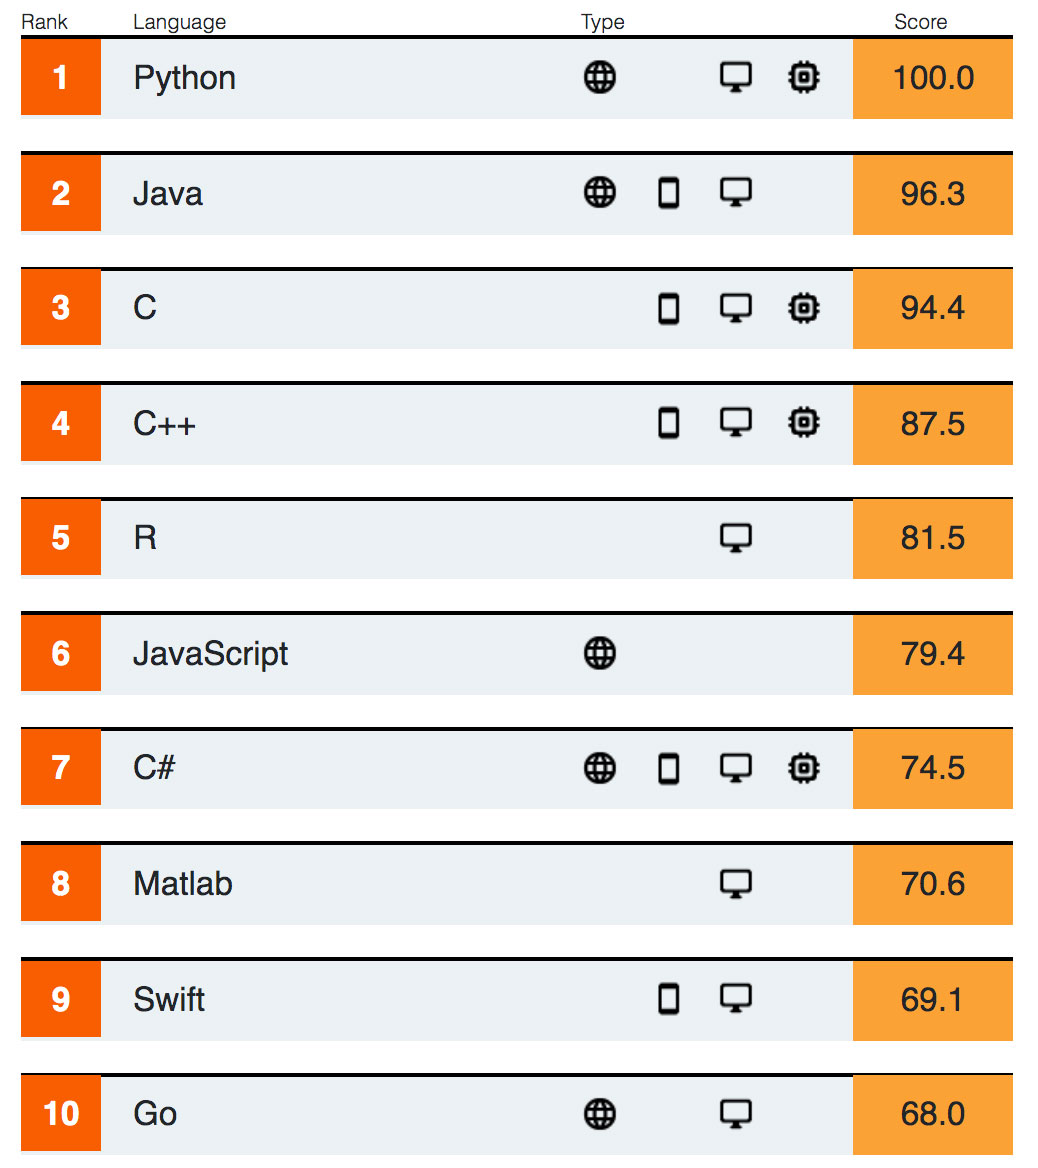
\includegraphics[width=4.6875in,height=\textheight]{images/01/topproglang.jpeg}

Despite being a much more specialized language than the others, it's maintained its popularity in recent years due to the world being awash in an ever-growing pile of big data.
\url{https://spectrum.ieee.org/computing/software/the-top-programming-languages-2019}

R은 통계분석에 널리 사용되는데 이는 데이터 가시화를 위한 그래픽 기능이나 벡터 연산 등의 편리함 때문에 점점 더 많은 사람들이 사용하고 있습니다. 기존에는 느린 속도나 부족한 확장성이 다른 언어들에 비해 단점으로 지적되었으나 R 언어의 계속적인 개발과 업데이트로 이러한 단점들이 빠르게 극복되고 있습니다. R 사용을 위해서는 R 언어의 코어 프로그램을 먼저 설치하고 그 다음 R 언어용 IDE인 RStudio 설치가 필요합니다.

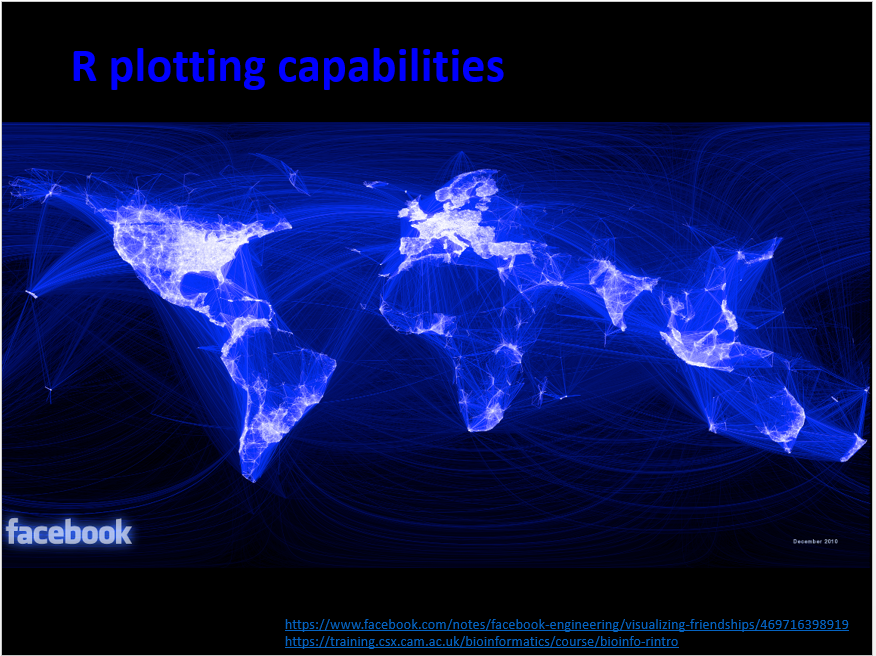
\includegraphics{images/01/22.PNG}

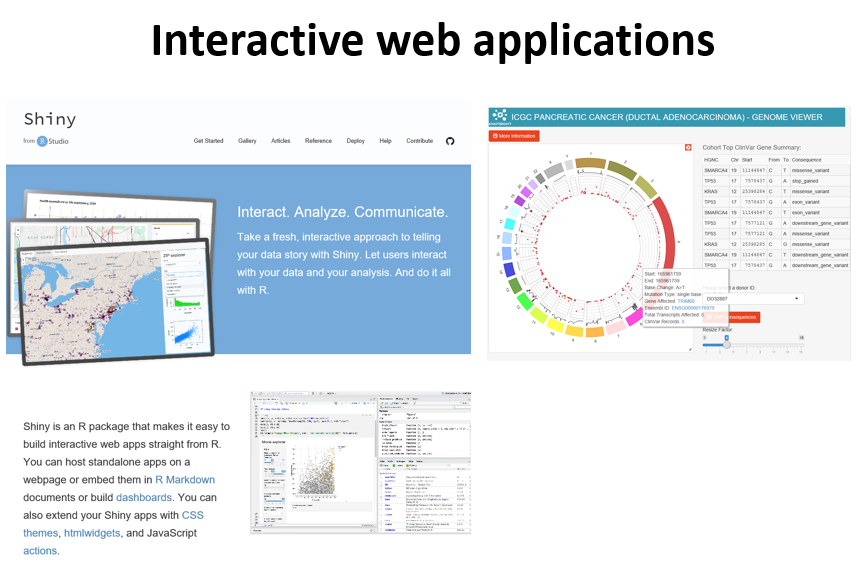
\includegraphics{images/01/23.PNG}

\hypertarget{r-rstudio-installation}{%
\section{R / Rstudio installation}\label{r-rstudio-installation}}

\hypertarget{r-uxc124uxce58}{%
\subsection{R 설치}\label{r-uxc124uxce58}}

\begin{itemize}
\tightlist
\item
  R 사이트에 접속 후 (\url{https://www.r-project.org/}) 좌측 메뉴 상단에 위치한 CRAN 클릭.
\item
  미러 사이트 목록에서 Korea의 아무 사이트나 들어감
\item
  Download R for Windows를 클릭 후 base 링크 들어가서
\item
  Download R x.x.x for Windows 링크 클릭으로 실행 프로그램 다운로드 - 로컬 컴퓨터에 Download 된 R-x.x.x-win.exe 를 실행
\item
  설치 가이드에 따라 R 언어 소프트웨어 설치 완료
\end{itemize}

\hypertarget{rstudio-uxc124uxce58}{%
\subsection{Rstudio 설치}\label{rstudio-uxc124uxce58}}

Rstudio는 R 언어를 위한 오픈소스 기반 통합개발환경(IDE)으로 R 프로그래밍을 위한 편리한 기능들을 제공해 줍니다.

\begin{itemize}
\tightlist
\item
  사이트에 접속 (\url{https://www.rstudio.com/}), 상단의 Products \textgreater{} RStudio 클릭
\item
  RStudio Desktop 선택
\item
  Download RStudio Desktop 클릭
\item
  RStudio Desktop Free 버전의 Download를 선택하고
\item
  Download RStudio for Windows 클릭, 다운로드
\item
  로컬 컴퓨터에 다운로드된 RStudio-x.x.x.exe 실행
\item
  설치 가이드에 따라 설치 완료
\end{itemize}

\hypertarget{rstudio-interface}{%
\section{Rstudio interface}\label{rstudio-interface}}

\begin{itemize}
\tightlist
\item
  좌측 상단의 공간은 코드편집창, 좌측 하단은 콘솔창 이며 각 위치를 기호에 따라서 바꿀 수 있습니다.
  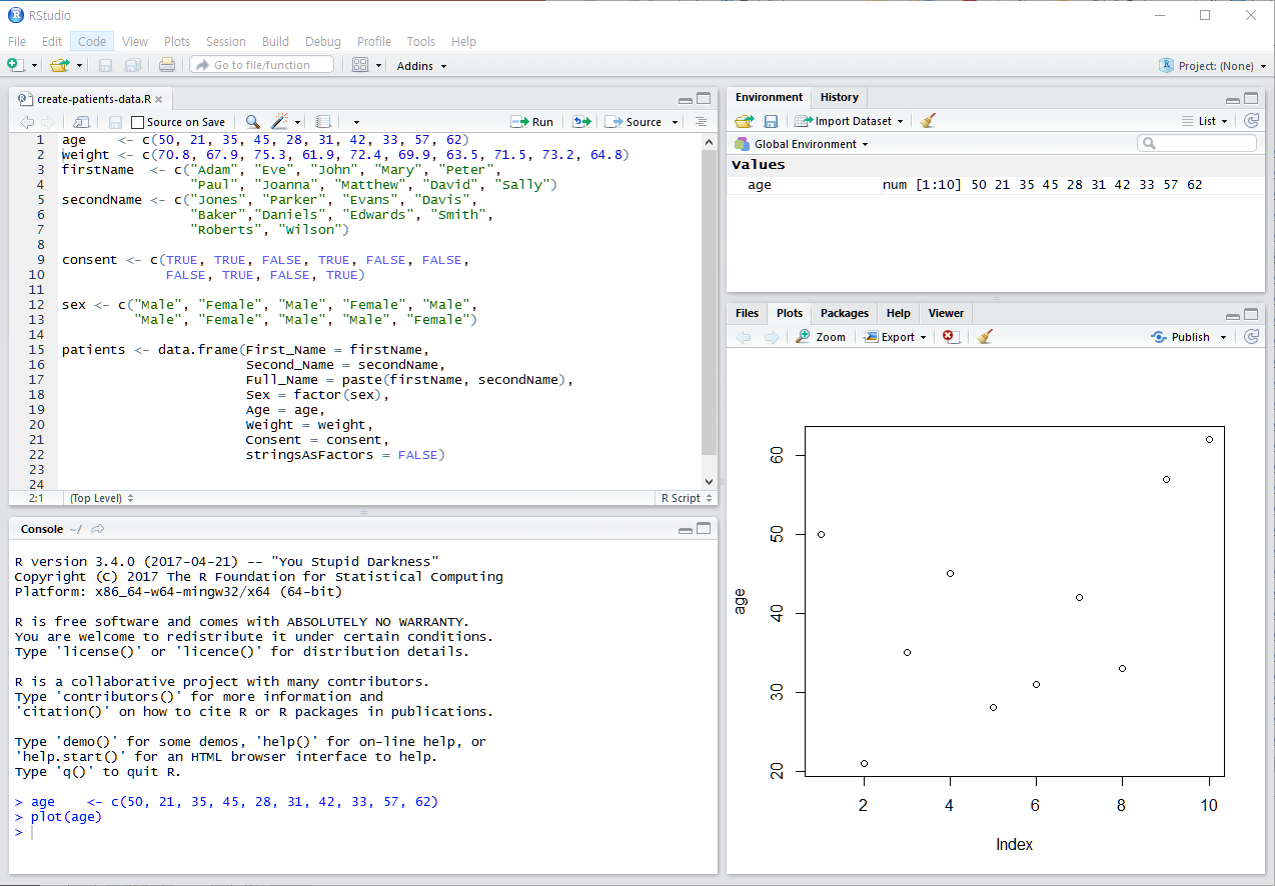
\includegraphics{images/01/01-11.PNG}
\end{itemize}

\hypertarget{keyboard-shortcuts}{%
\section{Keyboard shortcuts}\label{keyboard-shortcuts}}

\begin{itemize}
\tightlist
\item
  참고사이트

  \begin{itemize}
  \tightlist
  \item
    \url{https://support.rstudio.com/hc/en-us/articles/200711853-Keyboard-Shortcuts}
  \item
    Tools --\textgreater{} Keyboard shortcut Quick Reference (\texttt{Alt\ +\ Shift\ +\ K})
  \end{itemize}
\item
  코드편집창 이동 (\texttt{Ctrl+1}) 콘솔창 이동(\texttt{Ctrl+2})
\item
  한 줄 실행 (\texttt{Ctrl+Enter})
\item
  주석처리 (\texttt{Ctrl\ +\ Shift\ +\ C})

  \begin{itemize}
  \tightlist
  \item
    또는 \texttt{\#}으로 시작하는 라인
  \end{itemize}
\item
  실습

  \begin{itemize}
  \tightlist
  \item
    코드편집창에서 다음 입력
  \item
    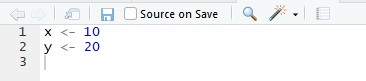
\includegraphics{images/01/01-14.PNG}\\
  \item
    단축키 \texttt{Ctrl\ +\ enter}로 코드 실행
  \item
    단축키 \texttt{Ctrl\ +\ 2}로 커서 콘솔창으로 이동
  \item
    \texttt{x}값 \texttt{x+y}값 확인
  \item
    단축키 \texttt{Ctrl\ +\ 1}로 코드편집창 이동
  \item
    단축키 \texttt{Ctrl\ +\ Shift\ +\ C} 사용
  \end{itemize}
\end{itemize}

\begin{Shaded}
\begin{Highlighting}[]
\CommentTok{\# x <{-} 10}
\CommentTok{\# y <{-} 20}
\end{Highlighting}
\end{Shaded}

\hypertarget{set-a-working-directory}{%
\section{Set a working directory}\label{set-a-working-directory}}

\begin{itemize}
\tightlist
\item
  시작 전 항상 작업 디렉토리 설정하는 것이 좋습니다. 예를 들어 \texttt{c:\textbackslash{}} 아래 새로운 디렉토리 rstat01 을 만들고 작업공간으로 설정할 수 있습니다.
\end{itemize}

\begin{Shaded}
\begin{Highlighting}[]
\KeywordTok{getwd}\NormalTok{()}
\KeywordTok{dir}\NormalTok{()}
\KeywordTok{setwd}\NormalTok{(}\StringTok{"C:}\CharTok{\textbackslash{}\textbackslash{}}\StringTok{rstat01"}\NormalTok{)}
\KeywordTok{getwd}\NormalTok{()}
\KeywordTok{dir}\NormalTok{()}
\end{Highlighting}
\end{Shaded}

\begin{itemize}
\tightlist
\item
  또는 RStudio \textgreater{} Session \textgreater{} Set Working Directory \textgreater{} Choose Directory
\end{itemize}

\hypertarget{set-a-project}{%
\section{Set a project}\label{set-a-project}}

\begin{itemize}
\item
  프로젝트를 만들어서 사용할 경우 파일이나 디렉토리, 내용 등을 쉽게 구분하여 사용 가능합니다. 아래와 같이 원하는 위치에 원하는 이름의 프로젝트를 생성하고 프로젝트를 시작할 때는 해당 디렉토리의 \texttt{xxx.Rproj} 파일을 클릭합니다.
\item
  File \textgreater{} New Project \textgreater{} New Directory \textgreater{}
\end{itemize}

\hypertarget{r-coding-practice}{%
\section{R coding practice}\label{r-coding-practice}}

\begin{itemize}
\tightlist
\item
  콘솔 계산기
\end{itemize}

\begin{Shaded}
\begin{Highlighting}[]
\DecValTok{2} \OperatorTok{+}\StringTok{ }\DecValTok{2}
\NormalTok{((}\DecValTok{2}\NormalTok{ – }\DecValTok{1}\NormalTok{)}\OperatorTok{\^{}}\DecValTok{2} \OperatorTok{+}\StringTok{ }\NormalTok{(}\DecValTok{1}\NormalTok{ – }\DecValTok{3}\NormalTok{)}\OperatorTok{\^{}}\DecValTok{2}\NormalTok{ )}\OperatorTok{\^{}}\NormalTok{(}\DecValTok{1}\OperatorTok{/}\DecValTok{2}\NormalTok{)}
\DecValTok{2} \OperatorTok{+}\StringTok{ }\DecValTok{2}\NormalTok{; }\DecValTok{2} \OperatorTok{{-}}\StringTok{ }\DecValTok{2}
\end{Highlighting}
\end{Shaded}

\begin{itemize}
\tightlist
\item
  Ex 1) 다음 공식들을 계산하는 R 코드를 작성하시오
\end{itemize}

\[
\sqrt{(4+3)(2+1)} \\
2^3 + 3^2 \\
\frac{0.25 - 0.2}{\sqrt{0.2 (1-0.2)/100}}
\]

\hypertarget{variables-and-values}{%
\section{Variables and values}\label{variables-and-values}}

\begin{itemize}
\tightlist
\item
  프로그래밍 언에어서 변수, 값 개념
\item
  Assignment operator ( \texttt{\textless{}-} OR \texttt{=} )

  \begin{itemize}
  \tightlist
  \item
    Valid object name \texttt{\textless{}-} value
  \item
    단축키: \texttt{Alt\ +\ -} (the minus sign)
  \end{itemize}
\end{itemize}

\begin{Shaded}
\begin{Highlighting}[]
\NormalTok{x <{-}}\StringTok{ }\DecValTok{2}
\NormalTok{y <{-}}\StringTok{ }\NormalTok{x}\OperatorTok{\^{}}\DecValTok{2}\NormalTok{ – }\DecValTok{2}\OperatorTok{*}\NormalTok{x }\OperatorTok{+}\StringTok{ }\DecValTok{1}
\NormalTok{y}
\NormalTok{x <{-}}\StringTok{ "two"}  
\NormalTok{some\_data <{-}}\StringTok{ }\FloatTok{9.8}
\end{Highlighting}
\end{Shaded}

\begin{itemize}
\tightlist
\item
  내장 변수 Built-in variables
\end{itemize}

\begin{Shaded}
\begin{Highlighting}[]
\NormalTok{pi}
\end{Highlighting}
\end{Shaded}

\begin{itemize}
\tightlist
\item
  변수이름 작명법

  \begin{itemize}
  \tightlist
  \item
    문자, 숫자, ``\_'', ``.'' 등으로 구성
  \item
    대소문자 구분
  \item
    가독성, 의미있는 변수 이름
  \item
    길이 제한 없음
  \end{itemize}
\end{itemize}

\begin{Shaded}
\begin{Highlighting}[]
\NormalTok{i\_use\_snake\_case <{-}}\StringTok{ }\DecValTok{1}
\NormalTok{otherPeopleUseCamelCase <{-}}\StringTok{ }\DecValTok{2}
\NormalTok{some.people.use.periods <{-}}\StringTok{ }\DecValTok{3}
\NormalTok{And\_aFew.People\_RENOUNCEconvention <{-}}\StringTok{ }\DecValTok{4}
\end{Highlighting}
\end{Shaded}

\begin{itemize}
\tightlist
\item
  자동 완성 기능 (Tab completion) in RStudio
\item
  이전 명령은 콘솔에서 위 아래 화살표
\end{itemize}

\hypertarget{variable-type-of-storage-mode}{%
\section{Variable type of (storage) mode}\label{variable-type-of-storage-mode}}

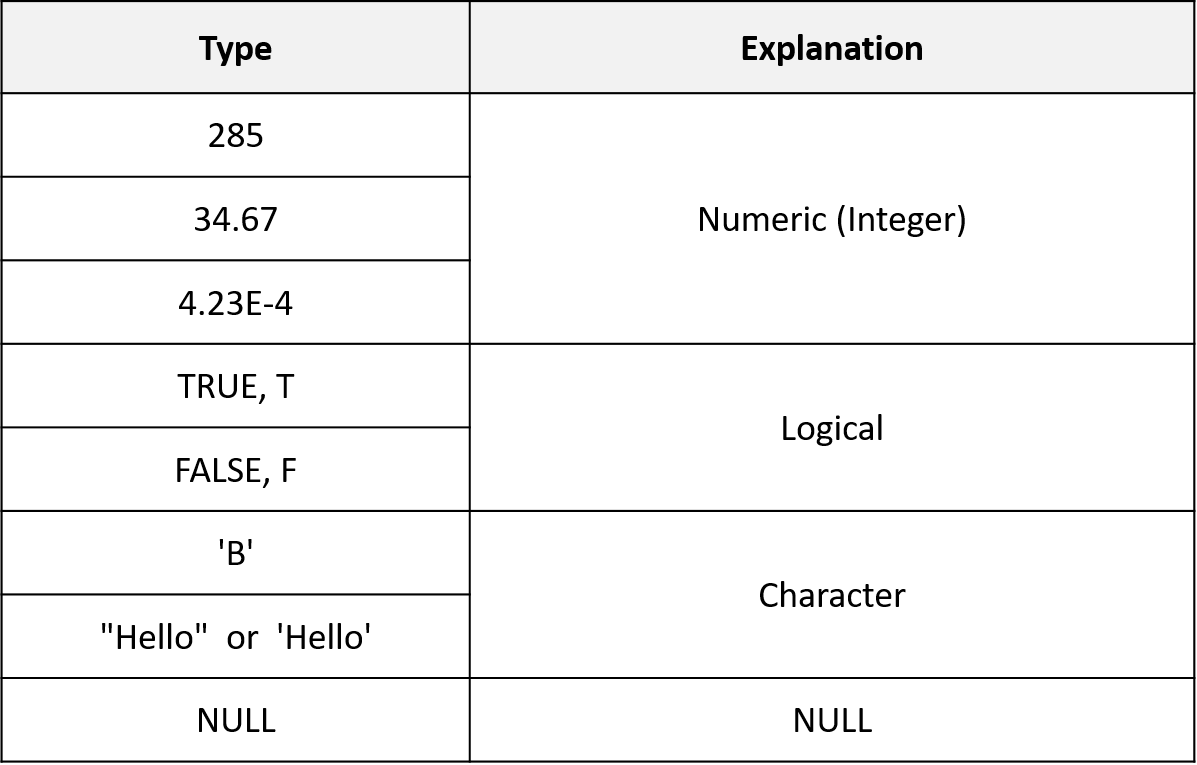
\includegraphics{images/01/01-13.PNG}

\hypertarget{variable---vectors}{%
\section{Variable - Vectors}\label{variable---vectors}}

\begin{itemize}
\tightlist
\item
  Combine function \texttt{c()}: Concatenating elements end to end
\end{itemize}

\begin{Shaded}
\begin{Highlighting}[]
\NormalTok{x <{-}}\StringTok{ }\KeywordTok{c}\NormalTok{(}\FloatTok{10.4}\NormalTok{, }\FloatTok{5.6}\NormalTok{, }\FloatTok{3.1}\NormalTok{, }\FloatTok{6.4}\NormalTok{, }\FloatTok{21.7}\NormalTok{) }
\NormalTok{y <{-}}\StringTok{ }\KeywordTok{c}\NormalTok{(}\StringTok{"X1"}\NormalTok{, }\StringTok{"Y2"}\NormalTok{,  }\StringTok{"X3"}\NormalTok{,  }\StringTok{"Y4"}\NormalTok{)}
\end{Highlighting}
\end{Shaded}

\hypertarget{indexing}{%
\section{Indexing}\label{indexing}}

\begin{itemize}
\tightlist
\item
  Subsets of the elements of a vector
\end{itemize}

\begin{Shaded}
\begin{Highlighting}[]
\NormalTok{x[}\DecValTok{1}\NormalTok{]}
\NormalTok{x[}\DecValTok{1}\OperatorTok{:}\DecValTok{3}\NormalTok{]}
\NormalTok{x[}\KeywordTok{c}\NormalTok{(}\DecValTok{1}\NormalTok{,}\DecValTok{2}\NormalTok{,}\DecValTok{4}\NormalTok{)]}
\NormalTok{y[}\DecValTok{3}\NormalTok{]}
\end{Highlighting}
\end{Shaded}

\hypertarget{functions}{%
\section{Functions}\label{functions}}

\begin{itemize}
\tightlist
\item
  함수 정의
\end{itemize}

\begin{Shaded}
\begin{Highlighting}[]
\NormalTok{my\_sine <{-}}\StringTok{ }\ControlFlowTok{function}\NormalTok{(x)\{}
\NormalTok{	y <{-}}\StringTok{ }\KeywordTok{sin}\NormalTok{(x)}
	\KeywordTok{return}\NormalTok{(y)}
\NormalTok{\}}
\end{Highlighting}
\end{Shaded}

\begin{itemize}
\tightlist
\item
  로딩 후 사용
\end{itemize}

\begin{Shaded}
\begin{Highlighting}[]
\KeywordTok{my\_sine}\NormalTok{(pi)}
\end{Highlighting}
\end{Shaded}

\begin{Shaded}
\begin{Highlighting}[]
\KeywordTok{log}\NormalTok{(}\DecValTok{100}\NormalTok{)}
\NormalTok{?log}
\KeywordTok{log}\NormalTok{(}\DecValTok{100}\NormalTok{, }\DataTypeTok{base=}\DecValTok{10}\NormalTok{)}
\KeywordTok{log}\NormalTok{(}\DecValTok{100}\NormalTok{, }\DecValTok{10}\NormalTok{)}
\end{Highlighting}
\end{Shaded}

\begin{itemize}
\tightlist
\item
  내장 함수 (Built-in functions)
\end{itemize}

\begin{Shaded}
\begin{Highlighting}[]
\NormalTok{x <{-}}\StringTok{ }\NormalTok{pi}
\KeywordTok{sin}\NormalTok{(x)}
\KeywordTok{sqrt}\NormalTok{(x)}
\KeywordTok{log}\NormalTok{(x)}
\KeywordTok{log}\NormalTok{(x, }\DecValTok{10}\NormalTok{)}
\NormalTok{x <{-}}\StringTok{ }\KeywordTok{c}\NormalTok{(}\DecValTok{10}\NormalTok{, }\DecValTok{20}\NormalTok{, }\DecValTok{30}\NormalTok{)}
\NormalTok{x }\OperatorTok{+}\StringTok{ }\NormalTok{x}
\KeywordTok{mean}\NormalTok{(x)}
\KeywordTok{sum}\NormalTok{(x)}\OperatorTok{/}\KeywordTok{length}\NormalTok{(x)}
\end{Highlighting}
\end{Shaded}

\hypertarget{vectorized-functions}{%
\section{Vectorized functions}\label{vectorized-functions}}

\begin{itemize}
\tightlist
\item
  백터연산은 R의 장점 중 하나로서 대부분의 함수들이 백터연산을 지원하고 이를 확장한 다양한 함수들을 사용하면 반복되는 프로세스를 빠르게 수행할 수 있습니다.
\end{itemize}

\begin{Shaded}
\begin{Highlighting}[]
\NormalTok{x <{-}}\StringTok{ }\KeywordTok{c}\NormalTok{(}\DecValTok{10}\NormalTok{, }\DecValTok{20}\NormalTok{, }\DecValTok{30}\NormalTok{)}
\NormalTok{x }\OperatorTok{+}\StringTok{ }\NormalTok{x}
\KeywordTok{sqrt}\NormalTok{(x)}
\KeywordTok{sin}\NormalTok{(x)}
\KeywordTok{log}\NormalTok{(x)}
\NormalTok{x}\OperatorTok{{-}}\KeywordTok{mean}\NormalTok{(x)}
\end{Highlighting}
\end{Shaded}

\hypertarget{help}{%
\section{Help}\label{help}}

\begin{Shaded}
\begin{Highlighting}[]
\NormalTok{?}
\NormalTok{?mean}
\KeywordTok{help}\NormalTok{(}\StringTok{"mean"}\NormalTok{)}
\KeywordTok{example}\NormalTok{(}\StringTok{"mean"}\NormalTok{)}
\KeywordTok{help.search}\NormalTok{(}\StringTok{"mean"}\NormalTok{)}
\KeywordTok{help}\NormalTok{(}\DataTypeTok{package=}\StringTok{"MASS"}\NormalTok{)}
\end{Highlighting}
\end{Shaded}

\hypertarget{r-packages}{%
\section{R packages}\label{r-packages}}

\begin{itemize}
\tightlist
\item
  R 패키지는 함수들의 모음으로 다른 사람들이 만들어 놓은 함수를 가져와서 사용할 수 있음
\item
  예) sum() 은 ``base'' package에 있고 sd() 함수는 ``stats'' package에서 제공
\item
  패키지를 구할 수 있는 가장 대표적인 사이트
\item
  The Comprehensive R Archive Network (CRAN) - \url{http://cran.r-project.org/web/views/}
\item
  Bioconductor - \url{http://www.bioconductor.org/packages/release/bioc/}
\end{itemize}

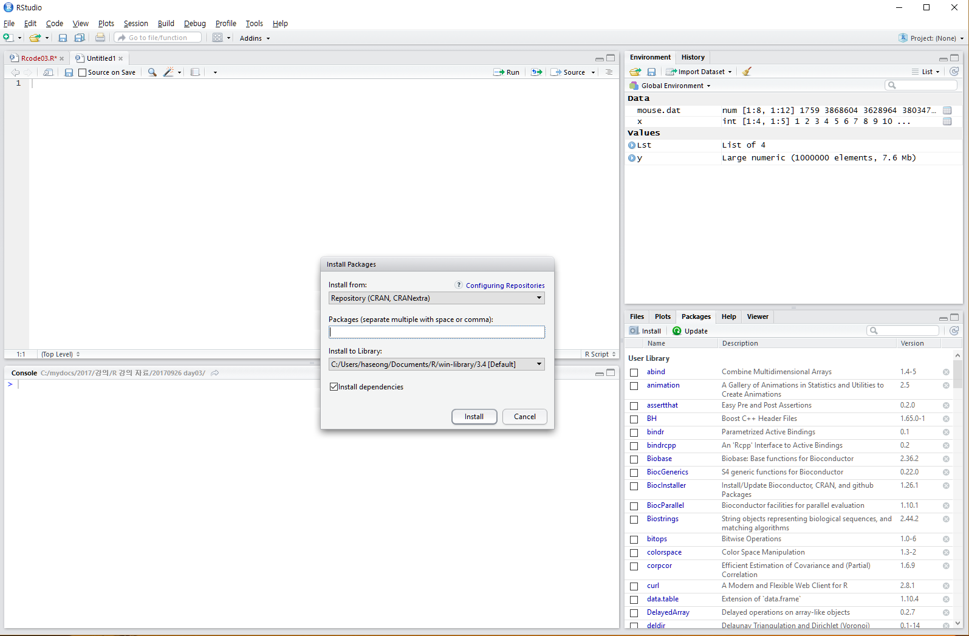
\includegraphics{images/01/01-18.png}

\begin{itemize}
\tightlist
\item
  UsingR package installation
\end{itemize}

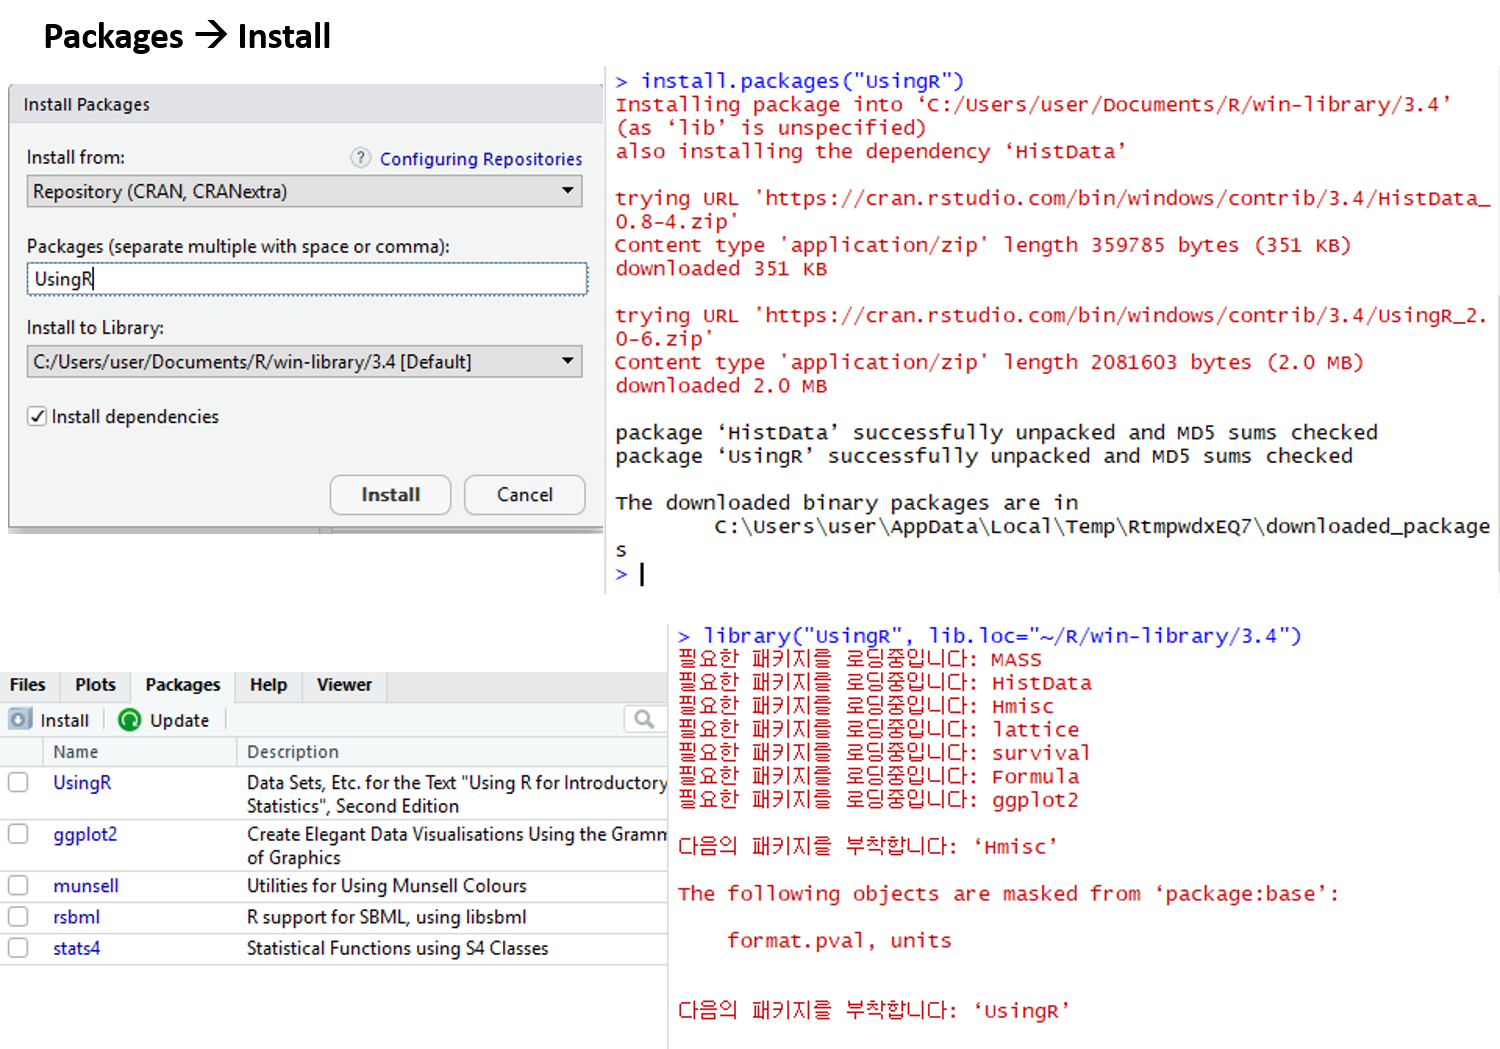
\includegraphics{images/01/01-19.png}

\begin{Shaded}
\begin{Highlighting}[]
\KeywordTok{install.packages}\NormalTok{(}\StringTok{"UsingR"}\NormalTok{)}
\end{Highlighting}
\end{Shaded}

\begin{itemize}
\tightlist
\item
  UsingR package loading
\end{itemize}

\begin{Shaded}
\begin{Highlighting}[]
\KeywordTok{library}\NormalTok{(UsingR)}
\KeywordTok{help}\NormalTok{(}\DataTypeTok{package=}\StringTok{"UsingR"}\NormalTok{)}
\end{Highlighting}
\end{Shaded}

\hypertarget{data-sets}{%
\section{Data sets}\label{data-sets}}

\begin{itemize}
\tightlist
\item
  일반적으로 패키지 안에 관련된 데이터도 같이 저장
\item
  data() function를 이용해서 패키지 데이터를 사용자 작업공간에 복사해서 사용 가능
\end{itemize}

\begin{Shaded}
\begin{Highlighting}[]
\KeywordTok{head}\NormalTok{(rivers)}
\KeywordTok{length}\NormalTok{(rivers)}
\KeywordTok{class}\NormalTok{(rivers)}
\KeywordTok{data}\NormalTok{(rivers)}
\KeywordTok{data}\NormalTok{(}\DataTypeTok{package=}\StringTok{"UsingR"}\NormalTok{)}
\KeywordTok{library}\NormalTok{(HistData)}
\KeywordTok{head}\NormalTok{(Cavendish)}
\KeywordTok{str}\NormalTok{(Cavendish)}
\KeywordTok{head}\NormalTok{(Cavendish}\OperatorTok{$}\NormalTok{density2)}
\end{Highlighting}
\end{Shaded}

\hypertarget{cheatsheet}{%
\section{Cheatsheet}\label{cheatsheet}}

\url{https://rstudio.com/resources/cheatsheets/}

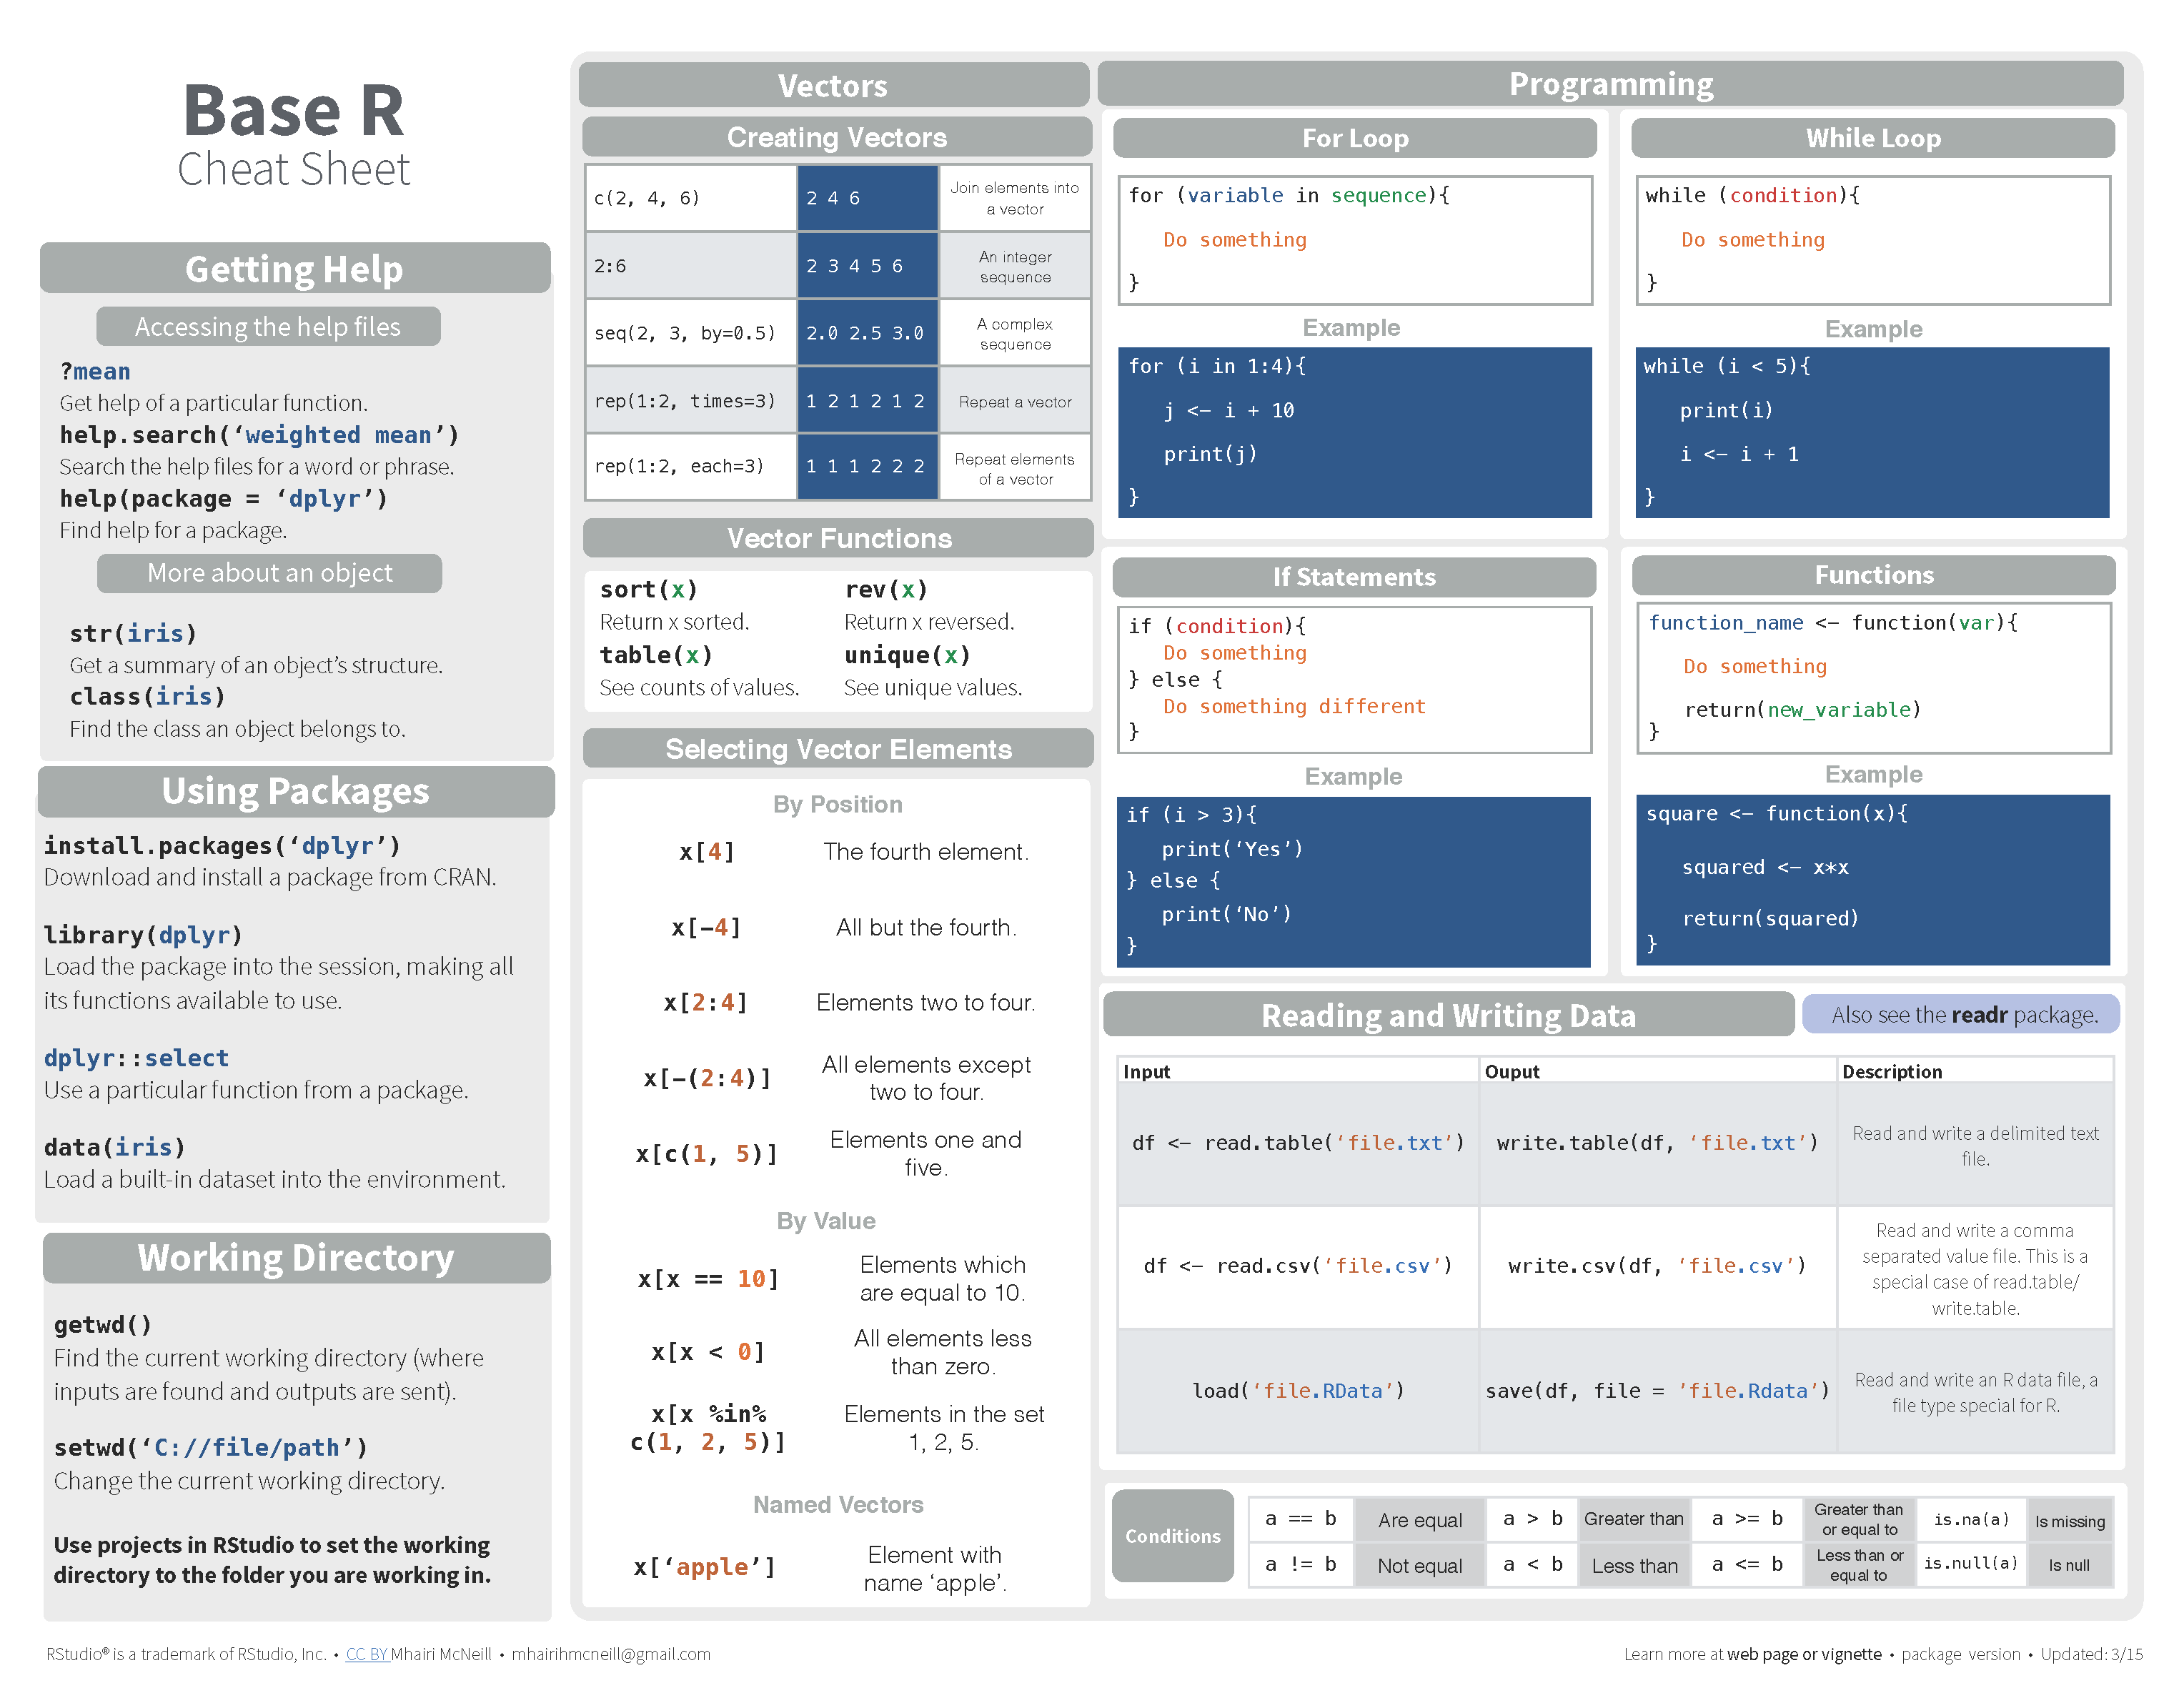
\includegraphics{images/01/base-r_1.png}
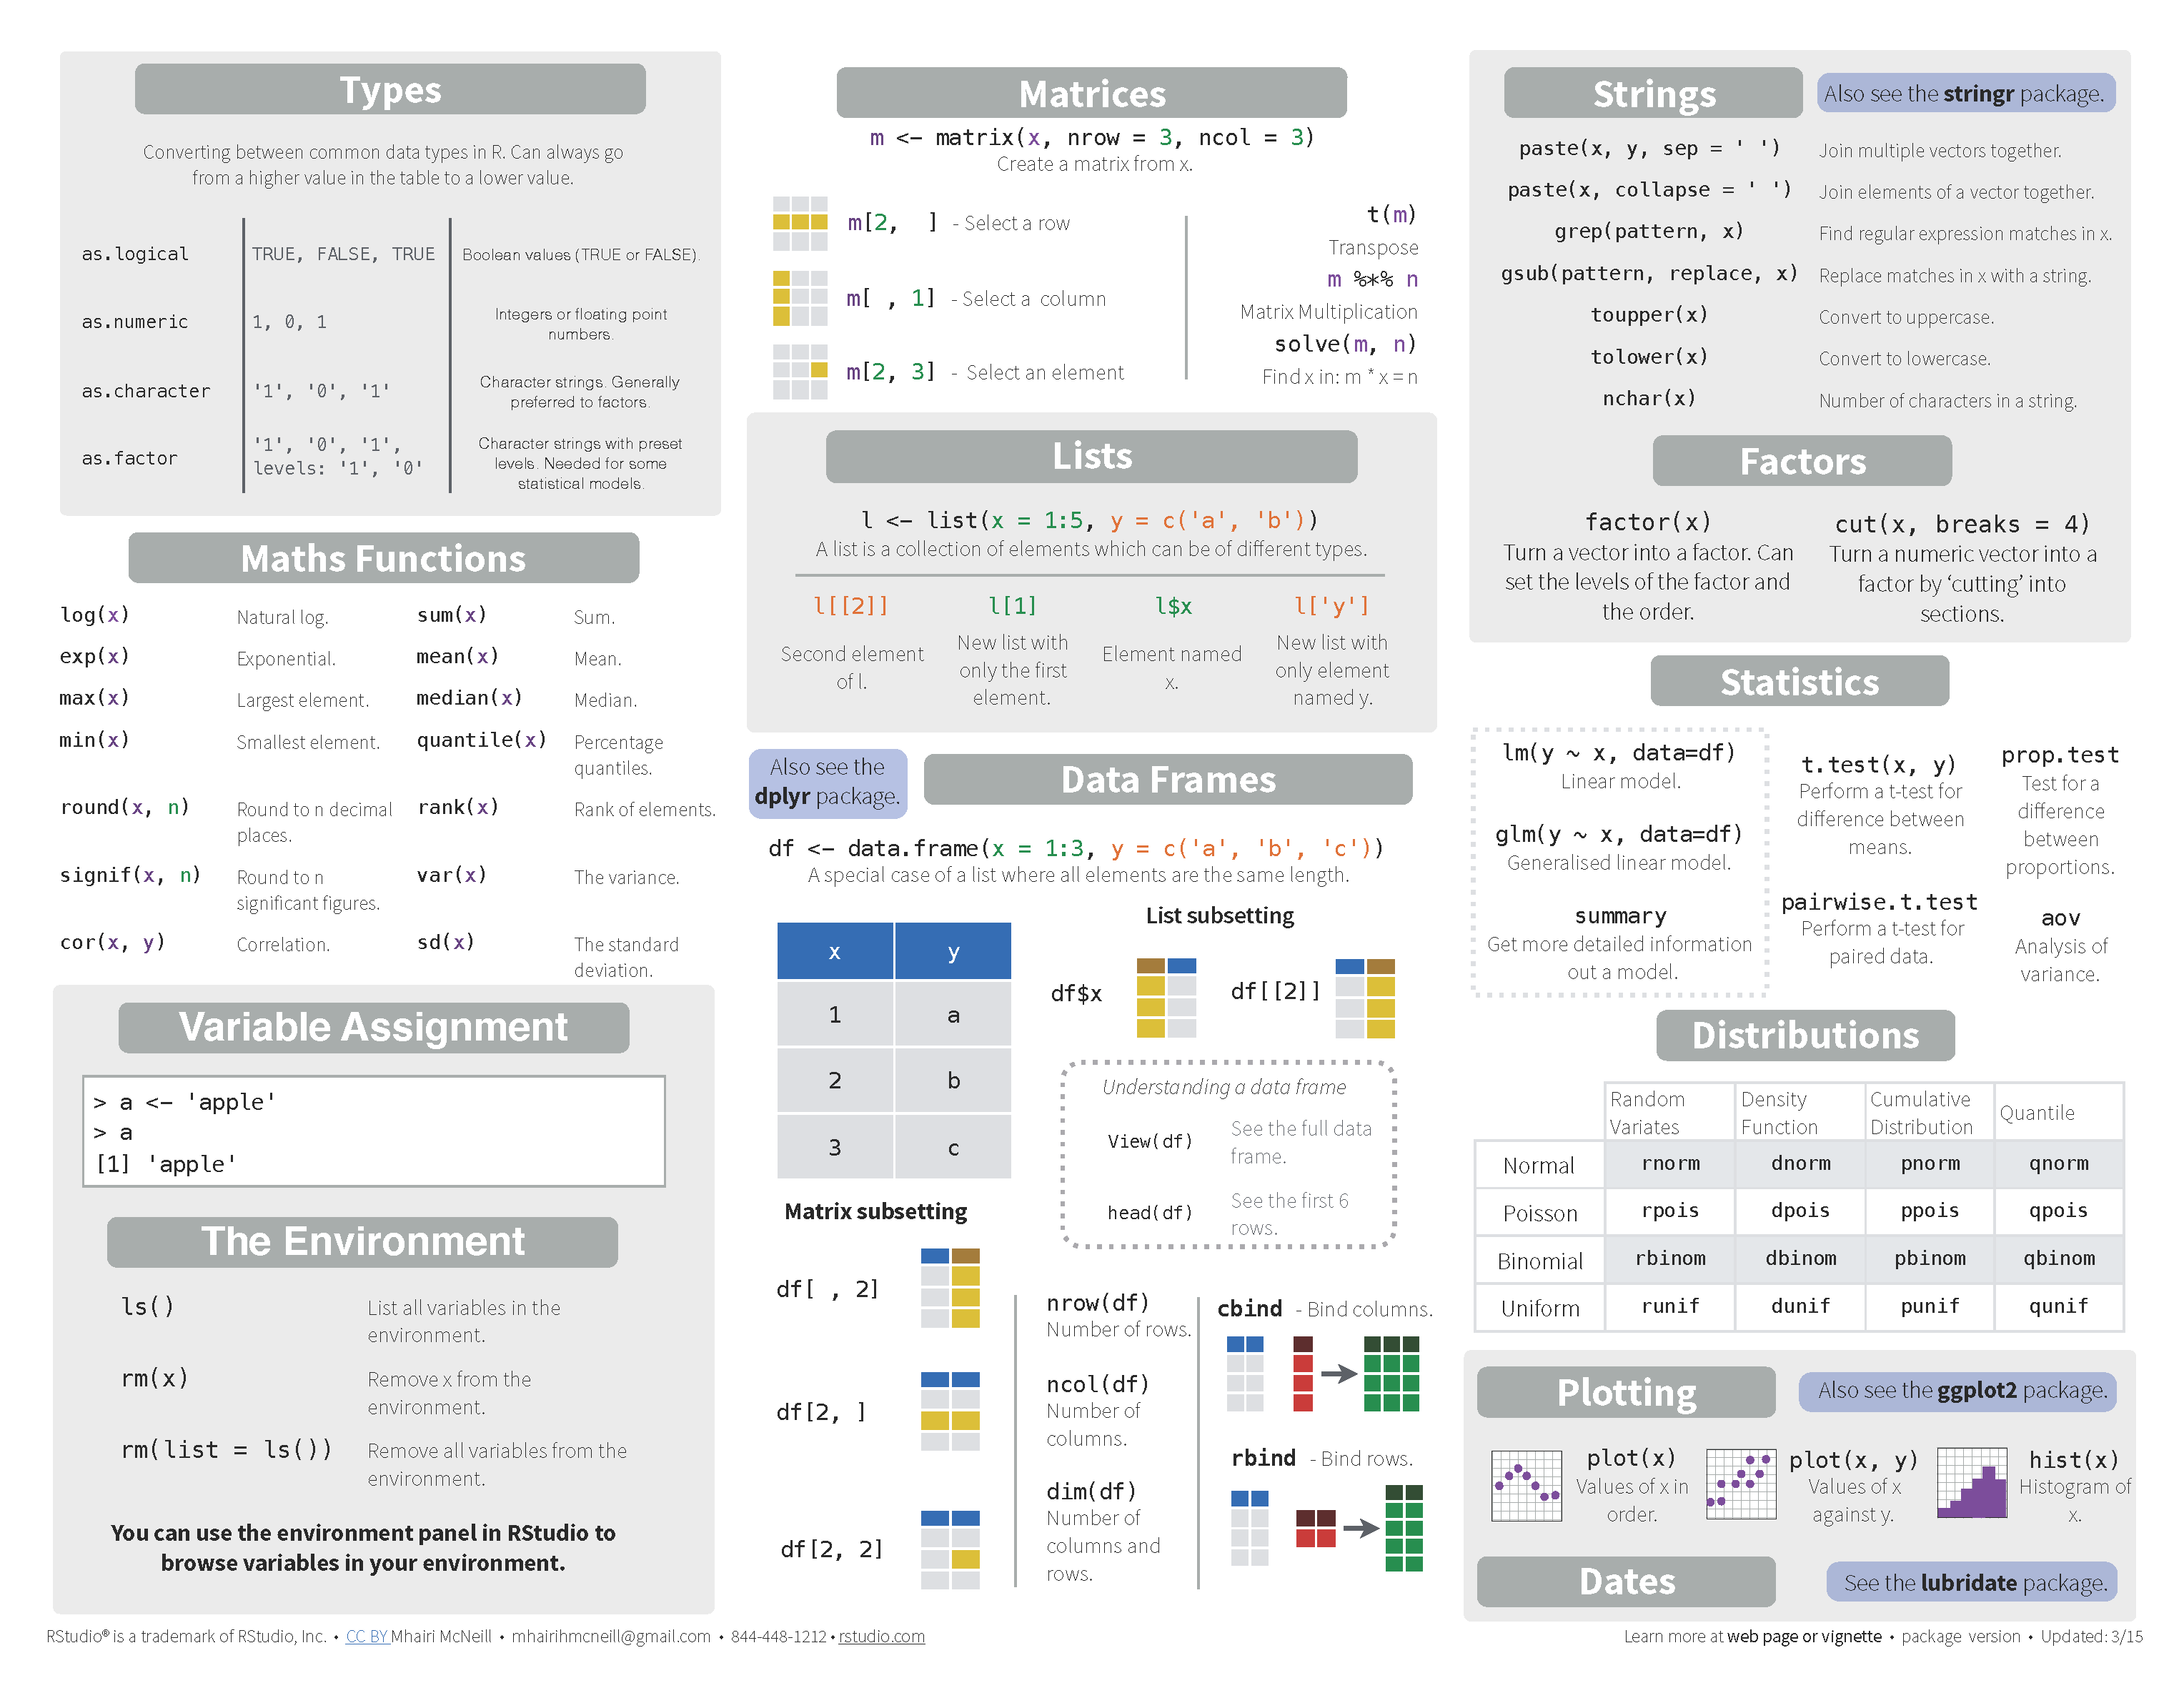
\includegraphics{images/01/base-r_2.png}

\hypertarget{problems}{%
\section{Problems}\label{problems}}

\begin{itemize}
\item
  1.2 변수 \texttt{x}에 1, 3, 5, 7, 9를 저장하는 코드를 작성하시오
\item
  1.3 변수 \texttt{y}에 2, 4, 6, 8, 10을 저장하는 코드를 작성하시오
\item
  1.4 위 변수 \texttt{x}와 \texttt{y}를 더한 값을 \texttt{z}에 저장하는 코드를 작성하시오 (백터연산)
\item
  1.5 \texttt{z}의 원소들의 합을 구하시오 (\texttt{sum()}함수 활용)
\item
  1.6 두 값을 입력받아 합을 출력하는 \texttt{mysum} 이름의 함수를 만들고 이 함수를 다음과 같이 이용해서 15와 20 두 값의 합을 구하는 코드를 작성하시오 (참고로 직접 만든 함수를 사용하기 위해서는 사용하기 전 해당 함수를 workspace에 등록하는 과정이 필요함)
\end{itemize}

\begin{Shaded}
\begin{Highlighting}[]
\NormalTok{z =}\StringTok{ }\KeywordTok{mysum}\NormalTok{(}\DecValTok{15}\NormalTok{, }\DecValTok{20}\NormalTok{)}
\KeywordTok{cat}\NormalTok{(z)}
\end{Highlighting}
\end{Shaded}

이 저작물은 크리에이티브 커먼즈 저작자표시-비영리-변경금지 4.0 국제 라이선스에 따라 이용할 수 있습니다.

\hypertarget{bioconductor}{%
\chapter{Bioconductor}\label{bioconductor}}

Bioconductor는 바이오인포메틱스를 위한 R기반의 데이터, 메소드, 그리고 패키지들의 모음입니다. 2002년 microarray 데이터 분석을 위한 플랫폼으로 시작되었으며 현재 1,300개 이상의 패키지로 구성되어 있습니다. R은 분산형 오픈소스이나 Bioconductor는 Full-time developer들에 의해서 유지되고 있습니다. \texttt{CRAN}에 배포되지 않고 \texttt{CRAN}에 비해 더 많은 필수 자료들 (vignettes 등)이 필요하며 높은 수준으로 quality control이 되고 있습니다. 현재 RNA-seq, ChIP seq, copy number analysis, microarray methylation, classic expression analysis, flow cytometry 등 다양한 분야의 데이터 분석에 사용되고 있습니다.

\textbf{특징}

Bioconductor 코어 개발 그룹은 사용자들이 지놈스케일 데이터를 더 편리하게 다루룰 수 있도록 데이터의 구조를 개발하는데 많은 시간을 들입니다.

\begin{itemize}
\tightlist
\item
  지놈스케일의 서열이나 발현등 대용량 데이터 관리\\
\item
  통계적 분석을 용이하게 수행하기 위한 전처리\\
\item
  분자수준의 현상과 생장이나 질병 등 표현형수준의 관계를 규명하기 위한 정량 데이터 통합\\
\item
  재사용 가능한 데이터를 위한 관리
\end{itemize}

\hypertarget{working-with-objects}{%
\section{Working with objects}\label{working-with-objects}}

객체지향프로그래밍 (OOP)은 복잡한 문제를 프로그래밍할 때 발생되는 코드의 복잡성을 해결할 수 있는 하나의 방안으로 1990년대부터 많이 사용되었습니다. Genome 스케일의 experiment나 annotation은 대표적인 복잡한 데이터 중 하나 입니다. \texttt{bioconcuctor}는 OOP의 개념을 도입하여 이러한 생물학 데이터를 구조화하고 효율적으로 데이터를 관리하고 있습니다.

\begin{Shaded}
\begin{Highlighting}[]
\CommentTok{\#\# it takes time at first}
\ControlFlowTok{if}\NormalTok{ (}\OperatorTok{!}\KeywordTok{requireNamespace}\NormalTok{(}\StringTok{"BiocManager"}\NormalTok{, }\DataTypeTok{quietly =} \OtherTok{TRUE}\NormalTok{))}
    \KeywordTok{install.packages}\NormalTok{(}\StringTok{"BiocManager"}\NormalTok{)}

\NormalTok{BiocManager}\OperatorTok{::}\KeywordTok{install}\NormalTok{(}\StringTok{"Homo.sapiens"}\NormalTok{)}
\end{Highlighting}
\end{Shaded}

Class와 Object, Instance 개념을 먼저 이해할 필요가 있습니다. 엄밀히 따지면 Object는 우리가 구현할 대상, Class는 설계도, Instance는 실제 구현한 대상 이라고 이해하시면 좋지만 가끔 Instance와 Object는 같은 의미로 사용되기도 합니다. 예를 들어 우리가 연구하는 \texttt{사람}, \texttt{원숭이}, \texttt{제브라피쉬} 라는 object들의 정보를 저장한다고 생각해 봅니다. 이 경우 각 객체들이 공통적으로 \texttt{gene}, \texttt{tRNA}, \texttt{rRNA} 등의 정보를 가지고 있고 그 기능적 annotation 또한 유사하므로 이러한 정보가 저장되는 공간을 갖는 \texttt{생명체}라는 개념적 설계도를 (Class) 먼저 만듭니다.

그리고 해당 클래스의 \texttt{사람}, \texttt{원숭이}, \texttt{제브라피쉬}를 만들면 각 객체를 일일히 구현할 필요 없이 필요한 정보를 미리 정해진 구조에 맞게 저장만 해주면 됩니다. 예를 들어 다음과 같습니다.

그런데 이러한 class가 무수히 존재하며 각 class마다 어떠한 정보가 있는지 알 수 없으므로 gene, tRNA 등의 정보에 접근할 수 있는 method들을 제공하고 있습니다. 예를 들어 객체 Homo.sapience를 살펴보면 다음과 같습니다.

\begin{Shaded}
\begin{Highlighting}[]
\KeywordTok{library}\NormalTok{(Homo.sapiens)}
\KeywordTok{class}\NormalTok{(Homo.sapiens)}
\KeywordTok{methods}\NormalTok{(}\DataTypeTok{class=}\KeywordTok{class}\NormalTok{(Homo.sapiens))}
\KeywordTok{genes}\NormalTok{(Homo.sapiens)}
\end{Highlighting}
\end{Shaded}

정리하면 bioconductor에는 대용량 정보가 object 형태로 구조화되어 저장되어 있으며 \texttt{library()}함수로 읽어올 수 있고 다양한 함수로 해당 object의 정보를 읽어올 수 있습니다.

\begin{Shaded}
\begin{Highlighting}[]
\KeywordTok{seqinfo}\NormalTok{(Homo.sapiens)}
\end{Highlighting}
\end{Shaded}

\hypertarget{discovering-installing-and-learning-how-to-use-bioconductor-packages}{%
\section{Discovering, installing, and learning how to use Bioconductor packages}\label{discovering-installing-and-learning-how-to-use-bioconductor-packages}}

\url{https://www.bioconductor.org}

\textbf{Discovery}

Use \textgreater\textgreater{} Software, Annotation, Experiment

\begin{itemize}
\tightlist
\item
  Software: 분석을 위한 툴 모음
\item
  Annotation: 유전자 symbol/ID mapping, gene ontology 기반 유전자 분류, 유전체상에서 exon, transcript, gene 등의 위치, 단백질 기능 등
\item
  Experiment data: 학습 가능할 정도의 Highly curated datasets (실험 데이터)
\item
  Workflow: 특정 데이터 분석을 위한 프로세스 모음
\end{itemize}

\textbf{Installation}

\texttt{BiocManager}를 먼저 설치하고 해당 패키지를 설치하시기 바랍니다. \texttt{BiocManager}에는 \texttt{available()}이라는 함수로 (특정 문자가 포함된) 사용 가능한 패키지를 검색할 수 도 있습니다.

Use \textgreater\textgreater{} Software \textgreater\textgreater{} IRanges

\begin{Shaded}
\begin{Highlighting}[]
\ControlFlowTok{if}\NormalTok{ (}\OperatorTok{!}\KeywordTok{requireNamespace}\NormalTok{(}\StringTok{"BiocManager"}\NormalTok{, }\DataTypeTok{quietly =} \OtherTok{TRUE}\NormalTok{))}
    \KeywordTok{install.packages}\NormalTok{(}\StringTok{"BiocManager"}\NormalTok{)}

\NormalTok{BiocManager}\OperatorTok{::}\KeywordTok{install}\NormalTok{(}\StringTok{"IRanges"}\NormalTok{)}
\CommentTok{\#\# .libPaths()}
\end{Highlighting}
\end{Shaded}

\textbf{Learning and support}

Learn \textgreater\textgreater{} Support site

\begin{Shaded}
\begin{Highlighting}[]
\KeywordTok{library}\NormalTok{(IRanges)}

\KeywordTok{vignette}\NormalTok{(}\DataTypeTok{package=}\StringTok{"IRanges"}\NormalTok{)}
\KeywordTok{browseVignettes}\NormalTok{(}\StringTok{"IRanges"}\NormalTok{)}
\KeywordTok{vignette}\NormalTok{(}\StringTok{"IRangesOverview"}\NormalTok{, }\DataTypeTok{package=}\StringTok{"IRanges"}\NormalTok{)}

\NormalTok{ir1 <{-}}\StringTok{ }\KeywordTok{IRanges}\NormalTok{(}\DataTypeTok{start=}\DecValTok{1}\OperatorTok{:}\DecValTok{10}\NormalTok{, }\DataTypeTok{width=}\DecValTok{10}\OperatorTok{:}\DecValTok{1}\NormalTok{)}
\NormalTok{ir1}
\KeywordTok{class}\NormalTok{(ir1)}
\KeywordTok{methods}\NormalTok{(}\DataTypeTok{class=}\StringTok{"IRanges"}\NormalTok{)}

\KeywordTok{example}\NormalTok{(IRanges)}
\NormalTok{?IRanges}
\NormalTok{??IRanges}
\end{Highlighting}
\end{Shaded}

\hypertarget{data-structure-and-management-for-genome-scale-experiments}{%
\section{Data structure and management for genome-scale experiments}\label{data-structure-and-management-for-genome-scale-experiments}}

잘못된 Data관리로 인한 손실을 줄이기 위해 고도로 효율적이고 신뢰성 높은 데이터 관리 툴이 필요합니다. 과학 연구에서 엑셀 기반의 데이터 관리는 신뢰성과 파이프라인 측면에서 적합하지 않습니다. 즉, 데이터를 관리하기 위해 특정 파이프라인을 만들고 이에 따라서 데이터를 관리할 때 높은 신뢰성의 데이터를 확보할 수 있고 과학적 추론의 바탕이 될 수 있습니다. 따라서 구조를 이해하고 어떻게 사용하는지를 알아야 합니다. Bioconductur에서는 지놈스케일 데이터를 모듈화하고 쉽게 확장 가능한 구조로 만들어서 사용합니다.

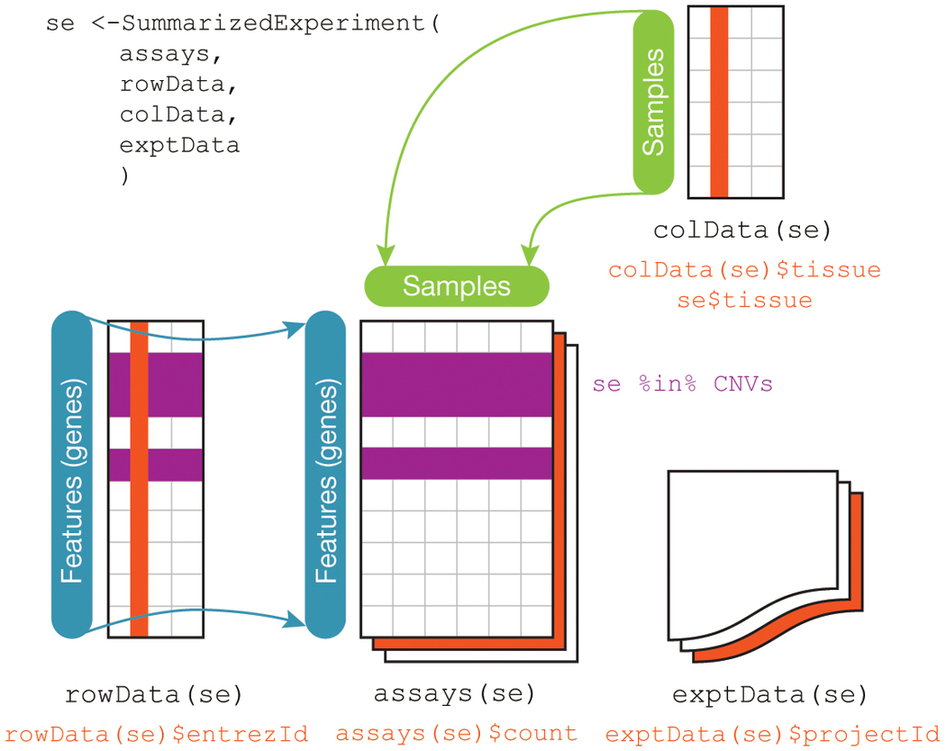
\includegraphics{images/bioconductor_strucure.jpg}

GEO 데이터를 예로 들어 보겠습니다.

\href{https://www.ncbi.nlm.nih.gov/geo/info/overview.html}{GEO설명} 참고

\href{https://www.bioconductor.org/packages/release/data/experiment/html/GSE62944.html}{GEO accession data GSE62944} 설명

\begin{Shaded}
\begin{Highlighting}[]
\ControlFlowTok{if}\NormalTok{ (}\OperatorTok{!}\KeywordTok{requireNamespace}\NormalTok{(}\StringTok{"BiocManager"}\NormalTok{, }\DataTypeTok{quietly =} \OtherTok{TRUE}\NormalTok{))}
    \KeywordTok{install.packages}\NormalTok{(}\StringTok{"BiocManager"}\NormalTok{)}

\NormalTok{BiocManager}\OperatorTok{::}\KeywordTok{install}\NormalTok{(}\StringTok{"GSE62944"}\NormalTok{)}
\KeywordTok{library}\NormalTok{(GSE62944)}
\KeywordTok{browseVignettes}\NormalTok{(}\StringTok{"GSE62944"}\NormalTok{)}

\NormalTok{BiocManager}\OperatorTok{::}\KeywordTok{install}\NormalTok{(}\StringTok{"ExperimentHub"}\NormalTok{)}
\KeywordTok{browseVignettes}\NormalTok{(}\StringTok{"ExperimentHub"}\NormalTok{)}
\KeywordTok{library}\NormalTok{(ExperimentHub)}

\NormalTok{eh =}\StringTok{ }\KeywordTok{ExperimentHub}\NormalTok{(}\DataTypeTok{localHub=}\OtherTok{FALSE}\NormalTok{)}

\KeywordTok{query}\NormalTok{(eh, }\StringTok{"GSE62944"}\NormalTok{)}
\NormalTok{tcga\_data <{-}}\StringTok{ }\NormalTok{eh[[}\StringTok{"EH1043"}\NormalTok{]]}
\end{Highlighting}
\end{Shaded}

\begin{Shaded}
\begin{Highlighting}[]
\NormalTok{gds <{-}}\StringTok{ }\KeywordTok{getGEO}\NormalTok{(}\DataTypeTok{filename=}\KeywordTok{system.file}\NormalTok{(}\StringTok{"extdata/GDS507.soft.gz"}\NormalTok{,}\DataTypeTok{package=}\StringTok{"GEOquery"}\NormalTok{))}
\NormalTok{gsm <{-}}\StringTok{ }\KeywordTok{getGEO}\NormalTok{(}\DataTypeTok{filename=}\KeywordTok{system.file}\NormalTok{(}\StringTok{"extdata/GSM11805.txt.gz"}\NormalTok{,}\DataTypeTok{package=}\StringTok{"GEOquery"}\NormalTok{))}
\end{Highlighting}
\end{Shaded}

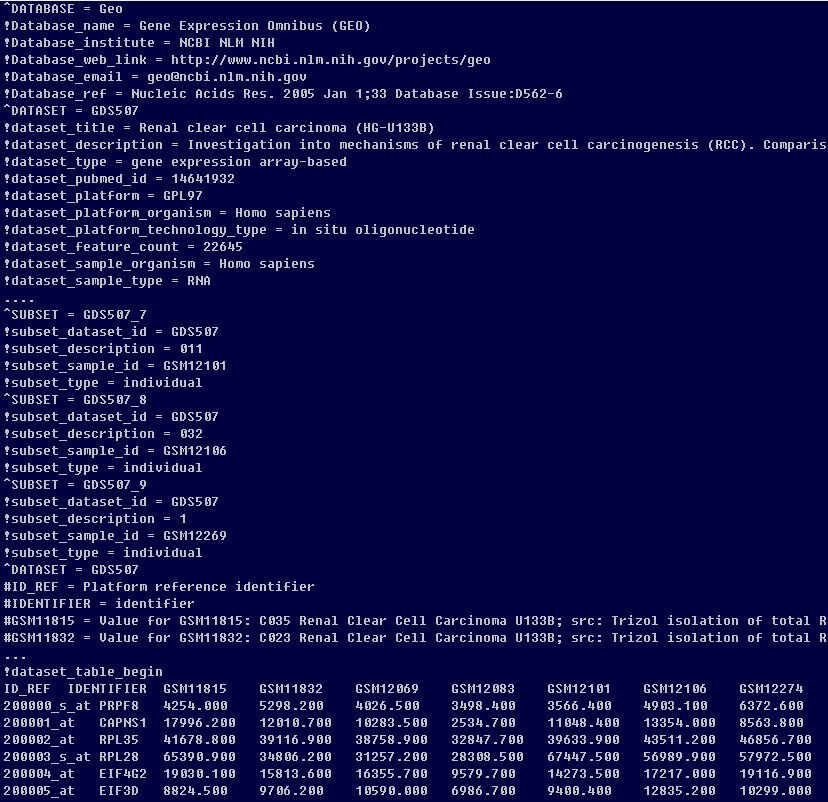
\includegraphics{images/geometa.JPG}

The Cancer Genome Atlas (TCGA): 암에 관한 유전변이 데이터를 통합 축적하고, 생물정보 분석 목적 (2005, Gene expression, SNP, CNV, DNA methylation, microRNA, Exome)

\hypertarget{object-variable-type-of-storage-mode}{%
\section{Object (variable) type of (storage) mode}\label{object-variable-type-of-storage-mode}}

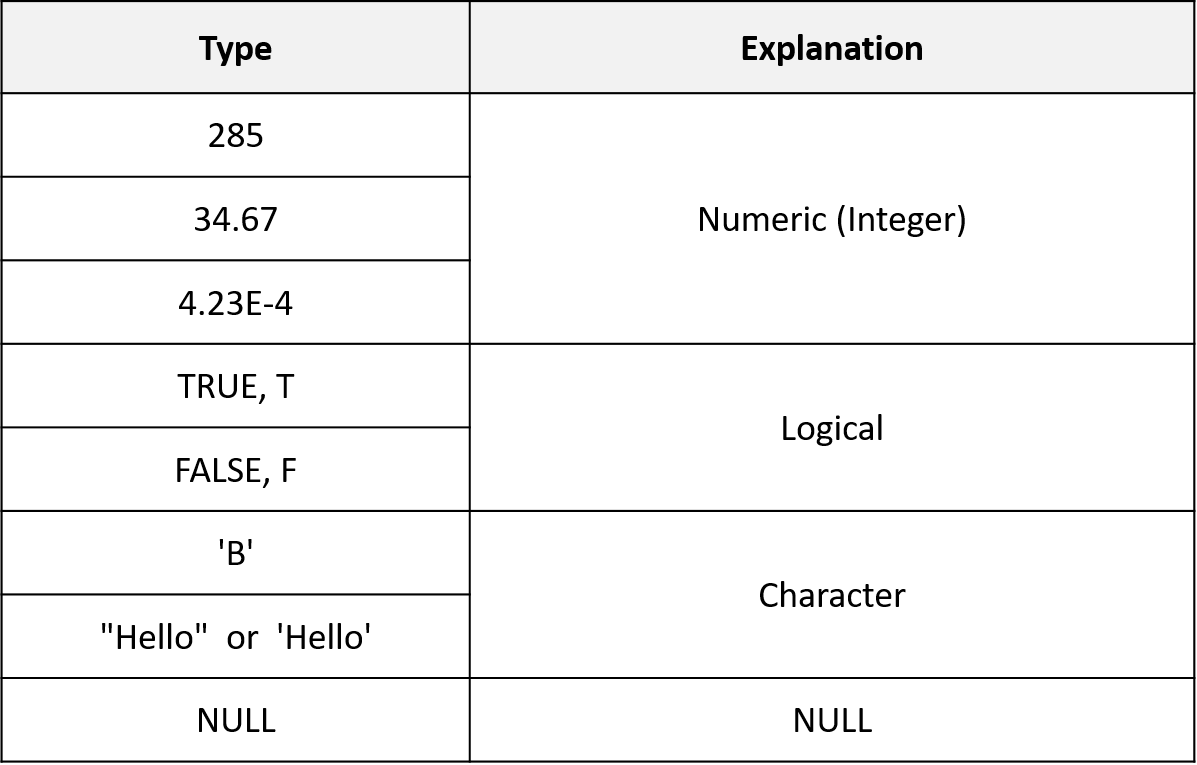
\includegraphics{images/01/01-13.PNG}

\hypertarget{levels-of-measurement}{%
\section{Levels of measurement}\label{levels-of-measurement}}

\begin{itemize}
\tightlist
\item
  Nominal (명목형) -- 사람 이름
\item
  Ordinal (순서형) -- 달리기 도착 순서
\item
  Interval (구간형) -- 선수1, 선수2 종점통과 시간
\item
  Ratio (비율형) -- 출발시간 기준 종점 통과 시간
\end{itemize}

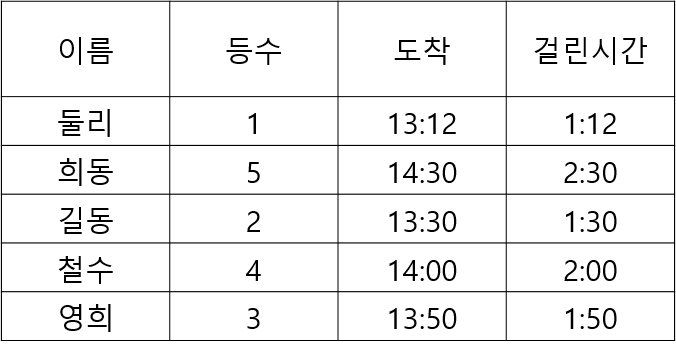
\includegraphics{images/02/01.png}

\begin{itemize}
\tightlist
\item
  Numeric data types

  \begin{itemize}
  \tightlist
  \item
    Discrete (이산형) data - 카운트, 횟수
  \item
    Continuous (연속형) data - 키, 몸무게, Cannot be shared
  \end{itemize}
\item
  Factors data - Categories to group the data
\item
  Character data - Identifiers
\item
  Date and time
\end{itemize}

\hypertarget{object---vectors}{%
\section{Object - Vectors}\label{object---vectors}}

\texttt{vector}는 R의 기본 데이터 구조입니다. numeric vector, logical vector, character vector 등 저장되는 값의 타입에 따라 크게 세가지로 나눌 수 있습니다. \texttt{class()} 함수를 이용해서 값의 타입을 알아낼 수 있습니다. Combine function인 \texttt{c()}를 활용하여 만들며 값을 순차적으로 붙여갈 수 있습니다.

\begin{Shaded}
\begin{Highlighting}[]
\NormalTok{x <{-}}\StringTok{ }\KeywordTok{c}\NormalTok{(}\FloatTok{10.4}\NormalTok{, }\FloatTok{5.6}\NormalTok{, }\FloatTok{3.1}\NormalTok{, }\FloatTok{6.4}\NormalTok{, }\FloatTok{21.7}\NormalTok{) }
\KeywordTok{class}\NormalTok{(x)}
\NormalTok{y <{-}}\StringTok{ }\KeywordTok{c}\NormalTok{(}\StringTok{"X1"}\NormalTok{, }\StringTok{"Y2"}\NormalTok{,  }\StringTok{"X3"}\NormalTok{,  }\StringTok{"Y4"}\NormalTok{)}
\KeywordTok{class}\NormalTok{(y)}
\NormalTok{z <{-}}\StringTok{ }\KeywordTok{c}\NormalTok{(T, F, F, T)}
\KeywordTok{class}\NormalTok{(z)}
\end{Highlighting}
\end{Shaded}

이 중 특히 numeric 형식의 벡터를 만드는 다양한 편의 함수들이 존재합니다.

\begin{Shaded}
\begin{Highlighting}[]
\DecValTok{1}\OperatorTok{:}\DecValTok{5}
\KeywordTok{seq}\NormalTok{(}\DecValTok{1}\NormalTok{,}\DecValTok{5}\NormalTok{, }\DataTypeTok{by=}\DecValTok{1}\NormalTok{)}
\KeywordTok{seq}\NormalTok{(}\DecValTok{0}\NormalTok{, }\DecValTok{100}\NormalTok{, }\DataTypeTok{by=}\DecValTok{10}\NormalTok{)}
\KeywordTok{seq}\NormalTok{(}\DecValTok{0}\NormalTok{, }\DecValTok{100}\NormalTok{, }\DataTypeTok{length.out=}\DecValTok{11}\NormalTok{)}
\NormalTok{?seq}

\KeywordTok{rep}\NormalTok{(}\DecValTok{5}\NormalTok{, }\DataTypeTok{times=}\DecValTok{10}\NormalTok{)}
\KeywordTok{rep}\NormalTok{(}\DecValTok{1}\OperatorTok{:}\DecValTok{3}\NormalTok{, }\DataTypeTok{times=}\DecValTok{4}\NormalTok{)}
\KeywordTok{rep}\NormalTok{(}\DecValTok{1}\OperatorTok{:}\DecValTok{3}\NormalTok{, }\DataTypeTok{each=}\DecValTok{3}\NormalTok{)}
\end{Highlighting}
\end{Shaded}

\hypertarget{exercise-3-1}{%
\subsection{Exercise 3-1}\label{exercise-3-1}}

odds라는 이름의 변수에 1부터 100까지의 홀수만을 저장하시오 (\texttt{seq()} 함수 사용)

\begin{center}\rule{0.5\linewidth}{0.5pt}\end{center}

\hypertarget{exercise-3-2}{%
\subsection{Exercise 3-2}\label{exercise-3-2}}

\texttt{1,\ 2,\ 3,\ 4,\ 5} 다섯 숫자에 대해서 두 개의 수를 뽑은 후 더해서 나올 수 있는 모든 수를 구하시오 즉, 1+1, 1+2, 1+3, \ldots, 2+1, 2+2, \ldots, 5+1, 5+2, \ldots, 5+5 의 모든 경우에 대한 결과값을 구함 (\texttt{rep()} 함수 사용)

\begin{center}\rule{0.5\linewidth}{0.5pt}\end{center}

Logical 벡터는 \texttt{True} 또는 \texttt{False}를 원소로 갖는 벡터 입니다. 앞글자가 대분자로 시작하는 것을 기억하시고 \texttt{T} 또는 \texttt{F}와 같이 한 문자로 표현할 수도 있습니다. 특정 조건에 대한 판단 결과를 반환할 경우에도 논리값을 사용합니다. 이 경우 조건을 판단 후 인덱싱 방법으로 해당 값들을 뽑아내기도 합니다.

\begin{Shaded}
\begin{Highlighting}[]
\KeywordTok{is.na}\NormalTok{(}\DecValTok{1}\NormalTok{)}
\KeywordTok{is.numeric}\NormalTok{(}\DecValTok{1}\NormalTok{)}
\KeywordTok{is.logical}\NormalTok{(}\OtherTok{TRUE}\NormalTok{)}

\NormalTok{x <{-}}\StringTok{ }\DecValTok{1}\OperatorTok{:}\DecValTok{20}
\NormalTok{x }\OperatorTok{>}\StringTok{ }\DecValTok{13}
\NormalTok{temp <{-}}\StringTok{ }\NormalTok{x }\OperatorTok{>}\StringTok{ }\DecValTok{13}
\KeywordTok{class}\NormalTok{(temp)}

\NormalTok{ages <{-}}\StringTok{ }\KeywordTok{c}\NormalTok{(}\DecValTok{66}\NormalTok{, }\DecValTok{57}\NormalTok{, }\DecValTok{60}\NormalTok{, }\DecValTok{41}\NormalTok{,  }\DecValTok{6}\NormalTok{, }\DecValTok{85}\NormalTok{, }\DecValTok{48}\NormalTok{, }\DecValTok{34}\NormalTok{, }\DecValTok{61}\NormalTok{, }\DecValTok{12}\NormalTok{)}
\NormalTok{ages }\OperatorTok{<}\StringTok{ }\DecValTok{30}
\KeywordTok{which}\NormalTok{(ages }\OperatorTok{<}\StringTok{ }\DecValTok{30}\NormalTok{)}
\NormalTok{i <{-}}\StringTok{ }\KeywordTok{which}\NormalTok{(ages }\OperatorTok{<}\StringTok{ }\DecValTok{30}\NormalTok{)}
\NormalTok{ages[i]}
\KeywordTok{any}\NormalTok{(ages }\OperatorTok{<}\StringTok{ }\DecValTok{30}\NormalTok{)}
\KeywordTok{all}\NormalTok{(ages }\OperatorTok{<}\StringTok{ }\DecValTok{30}\NormalTok{)}
\end{Highlighting}
\end{Shaded}

\hypertarget{exercise-3-3}{%
\subsection{Exercise 3-3}\label{exercise-3-3}}

1부터 100까지의 수를 n이라는 이름의 변수에 저장하고 이 중 짝수만을 뽑아내서 출력하시오 (\texttt{which()}함수 사용)

\begin{center}\rule{0.5\linewidth}{0.5pt}\end{center}

Character(문자형) 벡터의 경우 문자열을 다루는데 자주 쓰이는 \texttt{paste()} 함수의 사용법을 알아두면 편리합니다. \texttt{paste()} 함수는 서로 다른 문자열을 붙이는데 주로 사용됩니다. 참고로 문자열을 나누는 함수는 \texttt{strsplit()} 입니다. \texttt{paste()}에서 붙이는 문자 사이에 들어가는 문자를 지정하는 파라메터는 \texttt{sep} 이고 \texttt{strsplit()}함수에서 자르는 기준이 되는 문자는\texttt{split} 파라메터로 지정해 줍니다 (\texttt{?split} 또는 \texttt{?paste} 확인).

\begin{Shaded}
\begin{Highlighting}[]
\KeywordTok{paste}\NormalTok{(}\StringTok{"X"}\NormalTok{, }\StringTok{"Y"}\NormalTok{, }\StringTok{"Z"}\NormalTok{, }\DataTypeTok{sep=}\StringTok{"\_"}\NormalTok{)}
\KeywordTok{paste}\NormalTok{(}\KeywordTok{c}\NormalTok{(}\StringTok{"Four"}\NormalTok{,}\StringTok{"The"}\NormalTok{), }\KeywordTok{c}\NormalTok{(}\StringTok{"Score"}\NormalTok{,}\StringTok{"quick"}\NormalTok{), }\KeywordTok{c}\NormalTok{(}\StringTok{"and"}\NormalTok{,}\StringTok{"fox"}\NormalTok{), }\DataTypeTok{sep=}\StringTok{"\_"}\NormalTok{)}
\KeywordTok{paste}\NormalTok{(}\StringTok{"X"}\NormalTok{, }\DecValTok{1}\OperatorTok{:}\DecValTok{5}\NormalTok{, }\DataTypeTok{sep=}\StringTok{""}\NormalTok{)}
\KeywordTok{paste}\NormalTok{(}\KeywordTok{c}\NormalTok{(}\StringTok{"X"}\NormalTok{,}\StringTok{"Y"}\NormalTok{), }\DecValTok{1}\OperatorTok{:}\DecValTok{10}\NormalTok{, }\DataTypeTok{sep=}\StringTok{""}\NormalTok{)}

\NormalTok{x <{-}}\StringTok{ }\KeywordTok{c}\NormalTok{(}\StringTok{"X1"}\NormalTok{, }\StringTok{"Y2"}\NormalTok{, }\StringTok{"X3"}\NormalTok{, }\StringTok{"Y4"}\NormalTok{, }\StringTok{"X5"}\NormalTok{)}
\KeywordTok{paste}\NormalTok{(x[}\DecValTok{1}\NormalTok{], x[}\DecValTok{2}\NormalTok{])}
\KeywordTok{paste}\NormalTok{(x[}\DecValTok{1}\NormalTok{], x[}\DecValTok{2}\NormalTok{], }\DataTypeTok{sep=}\StringTok{""}\NormalTok{)}
\KeywordTok{paste}\NormalTok{(x, }\DataTypeTok{collapse=}\StringTok{"\_"}\NormalTok{)}

\KeywordTok{strsplit}\NormalTok{(}\StringTok{"XYZ"}\NormalTok{, }\DataTypeTok{split=}\StringTok{""}\NormalTok{)}
\end{Highlighting}
\end{Shaded}

Factor형은 범주형데이터를 저장하기 위한 object 이며 R 언어에서 특별히 만들어져 사용되고 있습니다. \texttt{factor()} 함수를 이용해 생성하며 생성된 객체는 다음과 같이 \texttt{level}이라는 범주를 나타내는 특성값을 가지고 있습니다.

\begin{Shaded}
\begin{Highlighting}[]
\NormalTok{x <{-}}\StringTok{ }\KeywordTok{c}\NormalTok{(}\StringTok{"Red"}\NormalTok{, }\StringTok{"Blue"}\NormalTok{, }\StringTok{"Yellow"}\NormalTok{, }\StringTok{"Green"}\NormalTok{, }\StringTok{"Blue"}\NormalTok{, }\StringTok{"Green"}\NormalTok{)}
\NormalTok{y <{-}}\StringTok{ }\KeywordTok{factor}\NormalTok{(x)}
\NormalTok{y}
\end{Highlighting}
\end{Shaded}

새로운 범주의 데이터를 추가할 경우 다음과 같이 해당되는 level을 먼저 추가하고 값을 저장해야 합니다.

\begin{Shaded}
\begin{Highlighting}[]
\KeywordTok{levels}\NormalTok{(y)}
\NormalTok{y[}\DecValTok{1}\NormalTok{] <{-}}\StringTok{ "Gold"}
\NormalTok{y}

\KeywordTok{levels}\NormalTok{(y) <{-}}\StringTok{ }\KeywordTok{c}\NormalTok{(}\KeywordTok{levels}\NormalTok{(y), }\StringTok{"Gold"}\NormalTok{)}
\KeywordTok{levels}\NormalTok{(y)}
\NormalTok{y}
\NormalTok{y[}\DecValTok{1}\NormalTok{] <{-}}\StringTok{ "Gold"}
\NormalTok{y}
\end{Highlighting}
\end{Shaded}

\texttt{factor}는 기본적으로 \texttt{level}에 표시된 순서가 위치 (정렬) 순서입니다. 이를 바꾸기 위해서는 다음과 같이 \texttt{levels} 함수를 이용해서 순서를 바꿀 수 있습니다.

\begin{Shaded}
\begin{Highlighting}[]
\CommentTok{\#library(UsingR)}
\KeywordTok{str}\NormalTok{(Cars93)}
\NormalTok{x <{-}}\StringTok{ }\NormalTok{Cars93}\OperatorTok{$}\NormalTok{Origin}
\KeywordTok{plot}\NormalTok{(x)}
\KeywordTok{levels}\NormalTok{(x) <{-}}\StringTok{ }\KeywordTok{c}\NormalTok{(}\StringTok{"non{-}USA"}\NormalTok{, }\StringTok{"USA"}\NormalTok{)}
\KeywordTok{levels}\NormalTok{(x)}
\KeywordTok{plot}\NormalTok{(x)}
\end{Highlighting}
\end{Shaded}

vector 들은 다음과 같은 builtin 함수들을 사용해서 해당 변수의 attribute를 알아낼 수 있습니다. attribute에는 원소 이름, 타입, 길이 등 vector형 변수가 가질 수 있는 특성을 말합니다.

\begin{Shaded}
\begin{Highlighting}[]
\KeywordTok{head}\NormalTok{(precip)}
\KeywordTok{class}\NormalTok{(precip)}
\KeywordTok{length}\NormalTok{(precip)}
\KeywordTok{names}\NormalTok{(precip)}

\NormalTok{test\_scores <{-}}\StringTok{ }\KeywordTok{c}\NormalTok{(}\DecValTok{100}\NormalTok{, }\DecValTok{90}\NormalTok{, }\DecValTok{80}\NormalTok{)}
\KeywordTok{names}\NormalTok{(test\_scores) <{-}}\StringTok{ }\KeywordTok{c}\NormalTok{(}\StringTok{"Alice"}\NormalTok{, }\StringTok{"Bob"}\NormalTok{, }\StringTok{"Shirley"}\NormalTok{)}
\NormalTok{test\_scores}
\end{Highlighting}
\end{Shaded}

인덱싱은 vector 데이터의 일부 데이터를 참조할 때 사용하는 방법입니다.

\begin{Shaded}
\begin{Highlighting}[]
\NormalTok{x[}\DecValTok{1}\NormalTok{]}
\NormalTok{x[}\DecValTok{1}\OperatorTok{:}\DecValTok{3}\NormalTok{]}
\NormalTok{i <{-}}\StringTok{ }\DecValTok{1}\OperatorTok{:}\DecValTok{3}
\NormalTok{x[i]}
\NormalTok{x[}\KeywordTok{c}\NormalTok{(}\DecValTok{1}\NormalTok{,}\DecValTok{2}\NormalTok{,}\DecValTok{4}\NormalTok{)]}
\NormalTok{y[}\DecValTok{3}\NormalTok{]}

\KeywordTok{head}\NormalTok{(precip)}
\NormalTok{precip[}\DecValTok{1}\NormalTok{]}
\NormalTok{precip[}\DecValTok{2}\OperatorTok{:}\DecValTok{10}\NormalTok{]}
\NormalTok{precip[}\KeywordTok{c}\NormalTok{(}\DecValTok{1}\NormalTok{,}\DecValTok{3}\NormalTok{,}\DecValTok{5}\NormalTok{)]}
\NormalTok{precip[}\OperatorTok{{-}}\DecValTok{1}\NormalTok{]}
\NormalTok{precip[}\StringTok{"Seattle Tacoma"}\NormalTok{]}
\NormalTok{precip[}\KeywordTok{c}\NormalTok{(}\StringTok{"Seattle Tacoma"}\NormalTok{, }\StringTok{"Portland"}\NormalTok{)]}
\NormalTok{precip[}\DecValTok{2}\NormalTok{] <{-}}\StringTok{ }\DecValTok{10}
\end{Highlighting}
\end{Shaded}

\hypertarget{object---matrix}{%
\section{Object - matrix}\label{object---matrix}}

매트릭스는 2차원 행렬로 같은 형식의 데이터 값 (numberic, character, logical) 으로만 채워진 행렬을 말합니다. 메트릭스를 만드는 방법은 아래와 같으며 \texttt{nrow} 와 \texttt{ncol} 파라메터에 행과 열의 수를 넣고 각 셀에 들어갈 값은 가장 앞에 위치한 data 파라메터에 넣어 줍니다 (\texttt{?matrix}로 파라메터 이름 확인). 메트릭스 인덱싱은 메트릭스 안의 값을 저장하거나 참조할때 (빼올때) 사용하는 방법입니다. 메트릭스 변수이름 바로 뒤에 대괄호를 이용해서 제어를 하며 대괄호 안에 콤마로 구분된 앞쪽은 row, 뒷쪽은 column 인덱스를 나타냅니다.

\begin{Shaded}
\begin{Highlighting}[]
\NormalTok{mymat <{-}}\StringTok{ }\KeywordTok{matrix}\NormalTok{(}\DecValTok{0}\NormalTok{, }\DataTypeTok{nrow=}\DecValTok{100}\NormalTok{, }\DataTypeTok{ncol=}\DecValTok{3}\NormalTok{) }\CommentTok{\# 1}
\NormalTok{mymat[,}\DecValTok{1}\NormalTok{] <{-}}\StringTok{ }\DecValTok{1}\OperatorTok{:}\DecValTok{100} \CommentTok{\# 2}
\NormalTok{mymat[,}\DecValTok{2}\NormalTok{] <{-}}\StringTok{ }\KeywordTok{seq}\NormalTok{(}\DecValTok{1}\NormalTok{,}\DecValTok{200}\NormalTok{,}\DecValTok{2}\NormalTok{) }\CommentTok{\# 3}
\NormalTok{mymat[,}\DecValTok{3}\NormalTok{] <{-}}\StringTok{ }\KeywordTok{seq}\NormalTok{(}\DecValTok{2}\NormalTok{,}\DecValTok{200}\NormalTok{,}\DecValTok{2}\NormalTok{) }\CommentTok{\# 4}
\end{Highlighting}
\end{Shaded}

매트릭스의 row나 column에 이름이 주어져 있을 경우 이름을 따옴표(")로 묶은 후 참조가 가능합니다. row나 column의 이름은 \texttt{rownames()} 또는 \texttt{colnames()}로 생성하거나 변경할 수 있습니다. row나 column의 개수는 \texttt{nrow()} 또는 \texttt{ncol()} 함수를 사용합니다.

\begin{Shaded}
\begin{Highlighting}[]
\KeywordTok{colnames}\NormalTok{(mymat)}
\KeywordTok{colnames}\NormalTok{(mymat) <{-}}\StringTok{ }\KeywordTok{c}\NormalTok{(}\StringTok{"A"}\NormalTok{, }\StringTok{"B"}\NormalTok{, }\StringTok{"C"}\NormalTok{)}
\KeywordTok{colnames}\NormalTok{(mymat)}
\KeywordTok{colnames}\NormalTok{(mymat)[}\DecValTok{2}\NormalTok{] <{-}}\StringTok{ "D"}
\KeywordTok{colnames}\NormalTok{(mymat)}
\KeywordTok{rownames}\NormalTok{(mymat) <{-}}\StringTok{ }\KeywordTok{paste}\NormalTok{(}\StringTok{"No"}\NormalTok{, }\DecValTok{1}\OperatorTok{:}\KeywordTok{nrow}\NormalTok{(mymat), }\DataTypeTok{sep=}\StringTok{""}\NormalTok{)}
\KeywordTok{rownames}\NormalTok{(mymat)}
\end{Highlighting}
\end{Shaded}

여러 row나 column을 참조할 경우 아래와 같이 combine 함수를 사용하여 묶어줘야 하며 스칼라값을 (임의의 숫자 하나) 더하거나 뺄 경우 vector / matrix 연산을 기본으로 수행합니다.

\begin{Shaded}
\begin{Highlighting}[]
\NormalTok{mymat[}\KeywordTok{c}\NormalTok{(}\DecValTok{2}\NormalTok{,}\DecValTok{3}\NormalTok{,}\DecValTok{4}\NormalTok{,}\DecValTok{5}\NormalTok{),}\DecValTok{2}\NormalTok{] }\CommentTok{\# 5}
\NormalTok{mymat}\DecValTok{{-}1} \CommentTok{\# 6}
\NormalTok{mysub <{-}}\StringTok{ }\NormalTok{mymat[,}\DecValTok{2}\NormalTok{] }\OperatorTok{{-}}\StringTok{ }\NormalTok{mymat[,}\DecValTok{1}\NormalTok{] }\CommentTok{\#7}
\KeywordTok{sum}\NormalTok{(mysub) }\CommentTok{\#8}
\KeywordTok{sum}\NormalTok{(mysub}\OperatorTok{\^{}}\DecValTok{2}\NormalTok{) }\CommentTok{\#8}
\end{Highlighting}
\end{Shaded}

\hypertarget{exercise-3-4}{%
\subsection{Exercise 3-4}\label{exercise-3-4}}

column이 3개이고 row가 3인 0으로 채워진 m이라는 이름의 matrix를 만들고 m의 각 원소를 1로 채우시오.

\begin{center}\rule{0.5\linewidth}{0.5pt}\end{center}

\hypertarget{object---data.frame}{%
\section{Object - data.frame}\label{object---data.frame}}

데이터프레임은 형태는 매트릭스와 같으나 컬럼 하나가 하나의 변수로서 각 변수들이 다른 모드의 값을 저장할 수 있다는 차이가 있습니다. \texttt{\$} 기호를 이용하여 각 구성 변수를 참조할 수 있습니다. 컬럼 한 줄이 하나의 변수 이므로 새로운 변수도 컬럼 형태로 붙여 넣을 수 있습니다. 즉, 각 row는 샘플을 나타내고 각 column은 변수를 나타내며 각 변수들이 갖는 샘플의 개수 (row의 길이, vector 의 길이)는 같아야 합니다. R 기반의 데이터 분석에서는 가장 선호되는 데이터 타입이라고 볼 수 있습니다.

\begin{Shaded}
\begin{Highlighting}[]
\CommentTok{\#\# data.frame}
\NormalTok{ids <{-}}\StringTok{ }\DecValTok{1}\OperatorTok{:}\DecValTok{10}
\NormalTok{ids}
\NormalTok{idnames <{-}}\StringTok{ }\KeywordTok{paste}\NormalTok{(}\StringTok{"Name"}\NormalTok{, ids, }\DataTypeTok{sep=}\StringTok{""}\NormalTok{)}
\NormalTok{idnames}
\NormalTok{students <{-}}\StringTok{ }\KeywordTok{data.frame}\NormalTok{(ids, idnames)}
\NormalTok{students}
\KeywordTok{class}\NormalTok{(students}\OperatorTok{$}\NormalTok{ids)}
\KeywordTok{class}\NormalTok{(students}\OperatorTok{$}\NormalTok{idnames)}
\NormalTok{students}\OperatorTok{$}\NormalTok{idnames}
\KeywordTok{str}\NormalTok{(students)}

\NormalTok{students <{-}}\StringTok{ }\KeywordTok{data.frame}\NormalTok{(ids, idnames, }\DataTypeTok{stringsAsFactors =}\NormalTok{ F)}
\KeywordTok{class}\NormalTok{(students}\OperatorTok{$}\NormalTok{idnames)}
\NormalTok{students}\OperatorTok{$}\NormalTok{idnames}
\NormalTok{students[}\DecValTok{1}\NormalTok{,]}
\KeywordTok{str}\NormalTok{(students)}
\end{Highlighting}
\end{Shaded}

데이터프레임에서도 변수 이름으로 인덱싱이 가능합니다.

\begin{Shaded}
\begin{Highlighting}[]
\CommentTok{\#\# data frame indexing }
\NormalTok{students}\OperatorTok{$}\NormalTok{ids}
\NormalTok{students[,}\DecValTok{1}\NormalTok{]}
\NormalTok{students[,}\StringTok{"ids"}\NormalTok{]}
\end{Highlighting}
\end{Shaded}

\hypertarget{object---list}{%
\section{Object - list}\label{object---list}}

리스트는 변수들의 모임이라는 점에서 데이터프레임과 같으나 구성 변수들의 길이가 모두 같아야 하는 데이터프레임과는 달리 다른 길이의 변수를 모아둘 수 있는 점이 다릅니다. 즉, R언어에서 두 변수를 담을 수 있는 데이터 타입은 \texttt{list}와 \texttt{data\ frame} 두 종류가 있는데 \texttt{list} 변수 타입은 \texttt{vector} 형태의 여러개의 element를 가질 수 있으며 각 \texttt{vector의} 길이가 모두 달라도 됩니다. list의 인덱싱에서 \texttt{{[}} \texttt{{]}}는 리스트를 반환하고 \texttt{{[}{[}} \texttt{{]}{]}}는 vector element들을 반환합니다.

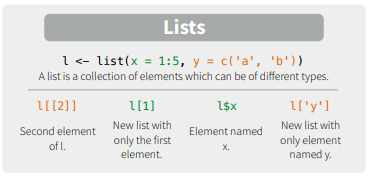
\includegraphics{images/03/05.PNG}

\begin{Shaded}
\begin{Highlighting}[]
\CommentTok{\#\# list}
\NormalTok{parent\_names <{-}}\StringTok{ }\KeywordTok{c}\NormalTok{(}\StringTok{"Fred"}\NormalTok{, }\StringTok{"Mary"}\NormalTok{)}
\NormalTok{number\_of\_children <{-}}\StringTok{ }\DecValTok{2}
\NormalTok{child\_ages <{-}}\StringTok{ }\KeywordTok{c}\NormalTok{(}\DecValTok{4}\NormalTok{, }\DecValTok{7}\NormalTok{, }\DecValTok{9}\NormalTok{)}
\KeywordTok{data.frame}\NormalTok{(parent\_names, number\_of\_children, child\_ages)}
\NormalTok{lst <{-}}\StringTok{ }\KeywordTok{list}\NormalTok{(parent\_names, number\_of\_children, child\_ages)}
\NormalTok{lst[}\DecValTok{1}\NormalTok{]}
\NormalTok{lst[[}\DecValTok{1}\NormalTok{]]}
\KeywordTok{class}\NormalTok{(lst[}\DecValTok{1}\NormalTok{])}
\KeywordTok{class}\NormalTok{(lst[[}\DecValTok{1}\NormalTok{]])}
\NormalTok{lst[[}\DecValTok{1}\NormalTok{]][}\DecValTok{1}\NormalTok{]}
\NormalTok{lst[[}\DecValTok{1}\NormalTok{]][}\KeywordTok{c}\NormalTok{(}\DecValTok{1}\NormalTok{,}\DecValTok{2}\NormalTok{)]}
\end{Highlighting}
\end{Shaded}

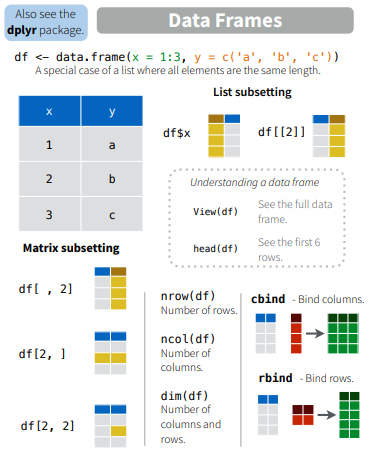
\includegraphics{images/03/06.PNG}

\hypertarget{missing-values}{%
\section{Missing values}\label{missing-values}}

특정 값이 ``Not available'' 이거나 ``Missing value'' 일 경우 벡터의 해당 원소 자리에 데이터의 이상을 알리기 위해 \texttt{NA}를 사용합니다. 따라서 일반적인 연산에서 \texttt{NA}가 포함되어 있는 경우 데이터의 불완전성을 알리기 위해 연산의 결과는 \texttt{NA}가 됩니다. \texttt{is.na()} 함수는 해당 변수에 \texttt{NA} 값이 있는지를 검사해주는 함수이며 R에는 이 외에도 다음과 같은 특수 값들이 사용되고 있습니다.

\begin{itemize}
\tightlist
\item
  NA: Not available, The value is missing
\item
  NULL: a reserved value
\item
  NaN: Not a number (0/0)
\item
  Inf: (1/0)
\end{itemize}

\begin{Shaded}
\begin{Highlighting}[]
\NormalTok{hip\_cost <{-}}\StringTok{ }\KeywordTok{c}\NormalTok{(}\DecValTok{10500}\NormalTok{, }\DecValTok{45000}\NormalTok{, }\DecValTok{74100}\NormalTok{, }\OtherTok{NA}\NormalTok{, }\DecValTok{83500}\NormalTok{)}
\KeywordTok{sum}\NormalTok{(hip\_cost)}
\KeywordTok{sum}\NormalTok{(hip\_cost, }\DataTypeTok{na.rm=}\OtherTok{TRUE}\NormalTok{)}
\NormalTok{?sum}
\end{Highlighting}
\end{Shaded}

\hypertarget{useful-functions-i}{%
\section{Useful functions I}\label{useful-functions-i}}

다음은 벡터형 변수와 같이 쓰이는 유용한 함수들입니다.

\begin{Shaded}
\begin{Highlighting}[]
\NormalTok{z <{-}}\StringTok{ }\KeywordTok{sample}\NormalTok{(}\DecValTok{1}\OperatorTok{:}\DecValTok{10}\NormalTok{, }\DecValTok{100}\NormalTok{, T)}
\KeywordTok{head}\NormalTok{(z)}
\KeywordTok{sort}\NormalTok{(z)}
\KeywordTok{order}\NormalTok{(z)}
\KeywordTok{table}\NormalTok{(z)}
\NormalTok{p <{-}}\StringTok{ }\NormalTok{z}\OperatorTok{/}\KeywordTok{sum}\NormalTok{(z)}
\KeywordTok{round}\NormalTok{(p, }\DataTypeTok{digits=}\DecValTok{1}\NormalTok{)}
\NormalTok{digits <{-}}\StringTok{ }\KeywordTok{as.character}\NormalTok{(z)}
\NormalTok{n <{-}}\StringTok{ }\KeywordTok{as.numeric}\NormalTok{(digits)}
\NormalTok{d <{-}}\StringTok{ }\KeywordTok{as.integer}\NormalTok{(digits)}
\end{Highlighting}
\end{Shaded}

\hypertarget{exercise-3-5}{%
\subsection{Exercise 3-5}\label{exercise-3-5}}

\begin{itemize}
\tightlist
\item
  score 라는 변수에 1부터 100까지 중 랜덤하게 선택된 20개의 수로 10 x 2 matrix를 만드시오
\item
  score의 row 이름을 문자형으로 Name1, Name2, \ldots, Name10으로 지정하시오 (\texttt{paste()}변수 사용)
\item
  score의 column 이름을 문자형으로 math와 eng로 지정하시오
\item
  이 matrix의 첫번째 컬럼과 두 번째 컬럼의 수를 각각 더한 후 total\_score라는 변수에 저장 하시오
\item
  total\_score 오름차순 순서를 나타내는 인덱스 (\texttt{order()}함수 사용)를 o라는 변수에 저장 하시오
\item
  score를 o순서로 재 배치 하고 score\_ordered 변수에 저장 하시오
\end{itemize}

\begin{center}\rule{0.5\linewidth}{0.5pt}\end{center}

이 저작물은 크리에이티브 커먼즈 저작자표시-비영리-변경금지 4.0 국제 라이선스에 따라 이용할 수 있습니다.

\hypertarget{r-programming-basics-i}{%
\chapter{R programming basics I}\label{r-programming-basics-i}}

\hypertarget{terminology}{%
\section{Terminology}\label{terminology}}

\begin{itemize}
\tightlist
\item
  Session: R 언어 실행 환경
\item
  Console: 명령어 입력하는 창
\item
  Code: R 프로그래밍 변수/제어문 모음
\item
  Objects (개체, variable): 데이터(값, value)가 저장되는 장소
\item
  Object (variable) types:

  \begin{itemize}
  \tightlist
  \item
    Vectors: 값들의 모임 combine function \texttt{c()} EX: c(6, 11, 13, 31, 90, 92)
  \item
    Factors: 범주형 데이터 저장 장소
  \item
    Data frames: 2D matrix 형태 데이터 자장 장소
  \end{itemize}
\item
  Data (value) types: Integers, doubles/numerics, logicals, and characters.
\item
  Conditionals (조건, 제어):

  \begin{itemize}
  \tightlist
  \item
    \texttt{if}, \texttt{==}, \texttt{\&} (AND), \texttt{\textbar{}} (OR) Ex: \texttt{(2\ +\ 1\ ==\ 3)\ \&\ (2\ +\ 1\ ==\ 4)}
  \item
    \texttt{for}, \texttt{while}: 반복 수
  \end{itemize}
\item
  Functions (함수, commands): 특정 일 수행, 함수이름 - 입력값 (arguments) - 출력값 (output) 으로 구성
\end{itemize}

\hypertarget{r-console-script}{%
\section{R console script}\label{r-console-script}}

콘솔에서 바로 계산을 수행할 수 있습니다. 참고로 이전에 수행한 명령은 콘솔에 커서가 있는 상태에서 위 아래 화살표를 누르면 볼 수 있고 엔터를 눌러 재사용 할 수 있습니다. \texttt{;}을 사용하면 두 개의 명령을 동시에 수행할 수 있습니다.

\[ 2 + 2 \]
\[ ((2 - 1)^2 + (1 - 3)^2)^{1/2} \]

\begin{Shaded}
\begin{Highlighting}[]
\DecValTok{2} \OperatorTok{+}\StringTok{ }\DecValTok{2}
\NormalTok{((}\DecValTok{2}\NormalTok{ – }\DecValTok{1}\NormalTok{)}\OperatorTok{\^{}}\DecValTok{2} \OperatorTok{+}\StringTok{ }\NormalTok{(}\DecValTok{1}\NormalTok{ – }\DecValTok{3}\NormalTok{)}\OperatorTok{\^{}}\DecValTok{2}\NormalTok{ )}\OperatorTok{\^{}}\NormalTok{(}\DecValTok{1}\OperatorTok{/}\DecValTok{2}\NormalTok{)}
\DecValTok{2} \OperatorTok{+}\StringTok{ }\DecValTok{2}\NormalTok{; }\DecValTok{2} \OperatorTok{{-}}\StringTok{ }\DecValTok{2}
\end{Highlighting}
\end{Shaded}

\hypertarget{what-is-a-programming-language}{%
\section{What is a programming language}\label{what-is-a-programming-language}}

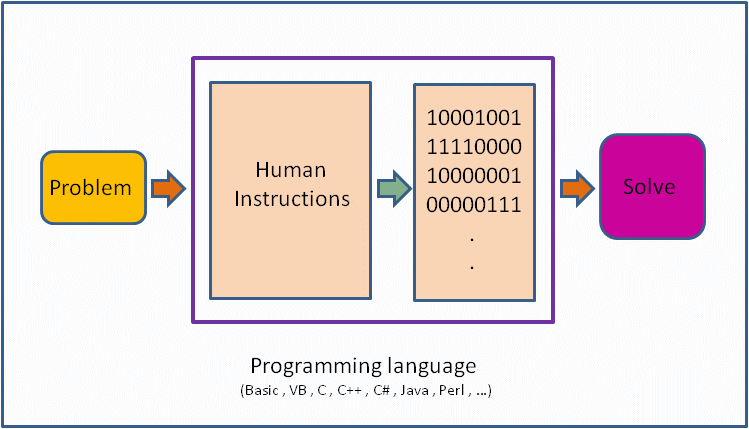
\includegraphics{images/01/24.PNG}
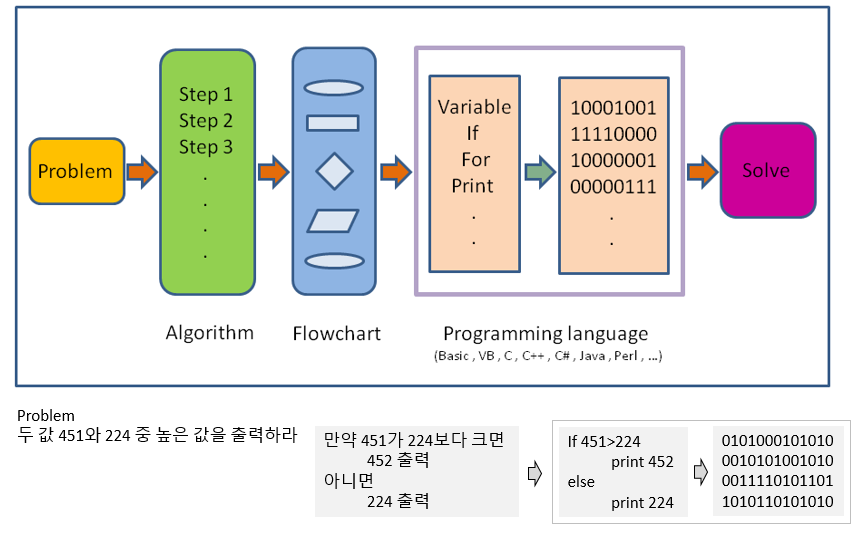
\includegraphics{images/01/25.PNG}

\hypertarget{variables-and-values}{%
\section{Variables and values}\label{variables-and-values}}

\begin{itemize}
\tightlist
\item
  R is a programming language
\item
  Assignment operator ( \texttt{\textless{}-} OR \texttt{=} )

  \begin{itemize}
  \tightlist
  \item
    Valid object name \texttt{\textless{}-} value
  \item
    단축키: \texttt{Alt\ +\ -} (the minus sign)
  \end{itemize}
\item
  내장 변수 Built-in variables
\end{itemize}

\begin{Shaded}
\begin{Highlighting}[]
\NormalTok{x <{-}}\StringTok{ }\DecValTok{2}
\NormalTok{y <{-}}\StringTok{ }\NormalTok{x}\OperatorTok{\^{}}\DecValTok{2}\NormalTok{ – }\DecValTok{2}\OperatorTok{*}\NormalTok{x }\OperatorTok{+}\StringTok{ }\DecValTok{1}
\NormalTok{y}
\NormalTok{x <{-}}\StringTok{ "two"}  
\NormalTok{some\_data <{-}}\StringTok{ }\FloatTok{9.8}
\NormalTok{pi}
\end{Highlighting}
\end{Shaded}

\begin{itemize}
\tightlist
\item
  변수이름 작명법

  \begin{itemize}
  \tightlist
  \item
    Characters (letters), numbers, ``\_'', ``.''
  \item
    A and a are different symbols
  \item
    Names are effectively unlimited in length
  \end{itemize}
\end{itemize}

\begin{Shaded}
\begin{Highlighting}[]
\NormalTok{i\_use\_snake\_case <{-}}\StringTok{ }\DecValTok{1}
\NormalTok{otherPeopleUseCamelCase <{-}}\StringTok{ }\DecValTok{2}
\NormalTok{some.people.use.periods <{-}}\StringTok{ }\DecValTok{3}
\NormalTok{And\_aFew.People\_RENOUNCEconvention <{-}}\StringTok{ }\DecValTok{4}
\end{Highlighting}
\end{Shaded}

\begin{itemize}
\tightlist
\item
  자동 완성 기능 (Tab completion) in RStudio
\end{itemize}

\hypertarget{object-variable-type-of-storage-mode}{%
\section{Object (variable) type of (storage) mode}\label{object-variable-type-of-storage-mode}}

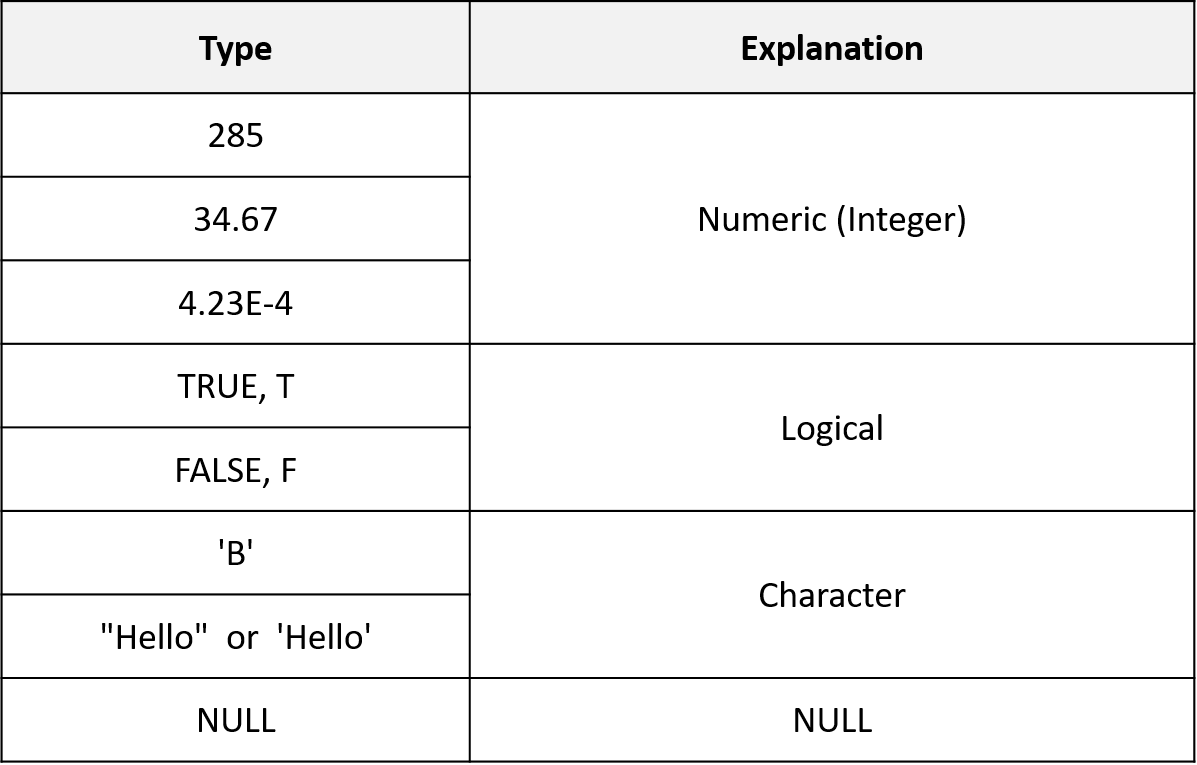
\includegraphics{images/01/01-13.PNG}

\hypertarget{levels-of-measurement}{%
\section{Levels of measurement}\label{levels-of-measurement}}

\begin{itemize}
\tightlist
\item
  Nominal (명목형) -- 사람 이름
\item
  Ordinal (순서형) -- 달리기 도착 순서
\item
  Interval (구간형) -- 선수1, 선수2 종점통과 시간
\item
  Ratio (비율형) -- 출발시간 기준 종점 통과 시간
\end{itemize}

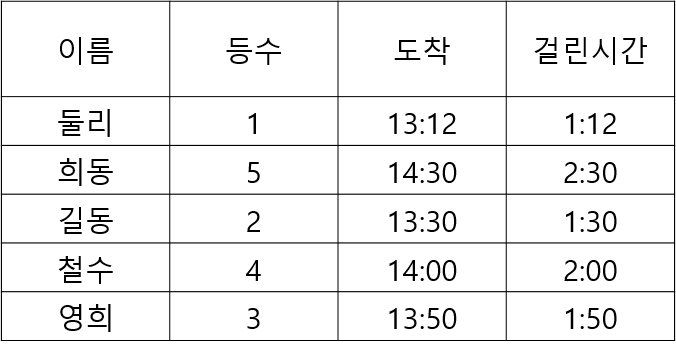
\includegraphics{images/02/01.png}

\begin{itemize}
\tightlist
\item
  Numeric data types

  \begin{itemize}
  \tightlist
  \item
    Discrete (이산형) data - 카운트, 횟수
  \item
    Continuous (연속형) data - 키, 몸무게, Cannot be shared
  \end{itemize}
\item
  Factors data - Categories to group the data
\item
  Character data - Identifiers
\item
  Date and time
\end{itemize}

\hypertarget{object---vectors}{%
\section{Object - Vectors}\label{object---vectors}}

\texttt{vector}는 R의 기본 데이터 구조입니다. numeric vector, logical vector, character vector 등 저장되는 값의 타입에 따라 크게 세가지로 나눌 수 있습니다. \texttt{class()} 함수를 이용해서 값의 타입을 알아낼 수 있습니다. Combine function인 \texttt{c()}를 활용하여 만들며 값을 순차적으로 붙여갈 수 있습니다.

\begin{Shaded}
\begin{Highlighting}[]
\NormalTok{x <{-}}\StringTok{ }\KeywordTok{c}\NormalTok{(}\FloatTok{10.4}\NormalTok{, }\FloatTok{5.6}\NormalTok{, }\FloatTok{3.1}\NormalTok{, }\FloatTok{6.4}\NormalTok{, }\FloatTok{21.7}\NormalTok{) }
\KeywordTok{class}\NormalTok{(x)}
\NormalTok{y <{-}}\StringTok{ }\KeywordTok{c}\NormalTok{(}\StringTok{"X1"}\NormalTok{, }\StringTok{"Y2"}\NormalTok{,  }\StringTok{"X3"}\NormalTok{,  }\StringTok{"Y4"}\NormalTok{)}
\KeywordTok{class}\NormalTok{(y)}
\NormalTok{z <{-}}\StringTok{ }\KeywordTok{c}\NormalTok{(T, F, F, T)}
\KeywordTok{class}\NormalTok{(z)}
\end{Highlighting}
\end{Shaded}

이 중 특히 numeric 형식의 벡터를 만드는 다양한 편의 함수들이 존재합니다.

\begin{Shaded}
\begin{Highlighting}[]
\DecValTok{1}\OperatorTok{:}\DecValTok{5}
\KeywordTok{seq}\NormalTok{(}\DecValTok{1}\NormalTok{,}\DecValTok{5}\NormalTok{, }\DataTypeTok{by=}\DecValTok{1}\NormalTok{)}
\KeywordTok{seq}\NormalTok{(}\DecValTok{0}\NormalTok{, }\DecValTok{100}\NormalTok{, }\DataTypeTok{by=}\DecValTok{10}\NormalTok{)}
\KeywordTok{seq}\NormalTok{(}\DecValTok{0}\NormalTok{, }\DecValTok{100}\NormalTok{, }\DataTypeTok{length.out=}\DecValTok{11}\NormalTok{)}
\NormalTok{?seq}

\KeywordTok{rep}\NormalTok{(}\DecValTok{5}\NormalTok{, }\DataTypeTok{times=}\DecValTok{10}\NormalTok{)}
\KeywordTok{rep}\NormalTok{(}\DecValTok{1}\OperatorTok{:}\DecValTok{3}\NormalTok{, }\DataTypeTok{times=}\DecValTok{4}\NormalTok{)}
\KeywordTok{rep}\NormalTok{(}\DecValTok{1}\OperatorTok{:}\DecValTok{3}\NormalTok{, }\DataTypeTok{each=}\DecValTok{3}\NormalTok{)}
\end{Highlighting}
\end{Shaded}

\hypertarget{exercise-3-1}{%
\subsection{Exercise 3-1}\label{exercise-3-1}}

odds라는 이름의 변수에 1부터 100까지의 홀수만을 저장하시오 (\texttt{seq()} 함수 사용)

\begin{center}\rule{0.5\linewidth}{0.5pt}\end{center}

\hypertarget{exercise-3-2}{%
\subsection{Exercise 3-2}\label{exercise-3-2}}

\texttt{1,\ 2,\ 3,\ 4,\ 5} 다섯 숫자에 대해서 두 개의 수를 뽑은 후 더해서 나올 수 있는 모든 수를 구하시오 즉, 1+1, 1+2, 1+3, \ldots, 2+1, 2+2, \ldots, 5+1, 5+2, \ldots, 5+5 의 모든 경우에 대한 결과값을 구함 (\texttt{rep()} 함수 사용)

\begin{center}\rule{0.5\linewidth}{0.5pt}\end{center}

Logical 벡터는 \texttt{True} 또는 \texttt{False}를 원소로 갖는 벡터 입니다. 앞글자가 대분자로 시작하는 것을 기억하시고 \texttt{T} 또는 \texttt{F}와 같이 한 문자로 표현할 수도 있습니다. 특정 조건에 대한 판단 결과를 반환할 경우에도 논리값을 사용합니다. 이 경우 조건을 판단 후 인덱싱 방법으로 해당 값들을 뽑아내기도 합니다.

\begin{Shaded}
\begin{Highlighting}[]
\KeywordTok{is.na}\NormalTok{(}\DecValTok{1}\NormalTok{)}
\KeywordTok{is.numeric}\NormalTok{(}\DecValTok{1}\NormalTok{)}
\KeywordTok{is.logical}\NormalTok{(}\OtherTok{TRUE}\NormalTok{)}

\NormalTok{x <{-}}\StringTok{ }\DecValTok{1}\OperatorTok{:}\DecValTok{20}
\NormalTok{x }\OperatorTok{>}\StringTok{ }\DecValTok{13}
\NormalTok{temp <{-}}\StringTok{ }\NormalTok{x }\OperatorTok{>}\StringTok{ }\DecValTok{13}
\KeywordTok{class}\NormalTok{(temp)}

\NormalTok{ages <{-}}\StringTok{ }\KeywordTok{c}\NormalTok{(}\DecValTok{66}\NormalTok{, }\DecValTok{57}\NormalTok{, }\DecValTok{60}\NormalTok{, }\DecValTok{41}\NormalTok{,  }\DecValTok{6}\NormalTok{, }\DecValTok{85}\NormalTok{, }\DecValTok{48}\NormalTok{, }\DecValTok{34}\NormalTok{, }\DecValTok{61}\NormalTok{, }\DecValTok{12}\NormalTok{)}
\NormalTok{ages }\OperatorTok{<}\StringTok{ }\DecValTok{30}
\KeywordTok{which}\NormalTok{(ages }\OperatorTok{<}\StringTok{ }\DecValTok{30}\NormalTok{)}
\NormalTok{i <{-}}\StringTok{ }\KeywordTok{which}\NormalTok{(ages }\OperatorTok{<}\StringTok{ }\DecValTok{30}\NormalTok{)}
\NormalTok{ages[i]}
\KeywordTok{any}\NormalTok{(ages }\OperatorTok{<}\StringTok{ }\DecValTok{30}\NormalTok{)}
\KeywordTok{all}\NormalTok{(ages }\OperatorTok{<}\StringTok{ }\DecValTok{30}\NormalTok{)}
\end{Highlighting}
\end{Shaded}

\hypertarget{exercise-3-3}{%
\subsection{Exercise 3-3}\label{exercise-3-3}}

1부터 100까지의 수를 n이라는 이름의 변수에 저장하고 이 중 짝수만을 뽑아내서 출력하시오 (\texttt{which()}함수 사용)

\begin{center}\rule{0.5\linewidth}{0.5pt}\end{center}

Character(문자형) 벡터의 경우 문자열을 다루는데 자주 쓰이는 \texttt{paste()} 함수의 사용법을 알아두면 편리합니다. \texttt{paste()} 함수는 서로 다른 문자열을 붙이는데 주로 사용됩니다. 참고로 문자열을 나누는 함수는 \texttt{strsplit()} 입니다. \texttt{paste()}에서 붙이는 문자 사이에 들어가는 문자를 지정하는 파라메터는 \texttt{sep} 이고 \texttt{strsplit()}함수에서 자르는 기준이 되는 문자는\texttt{split} 파라메터로 지정해 줍니다 (\texttt{?split} 또는 \texttt{?paste} 확인).

\begin{Shaded}
\begin{Highlighting}[]
\KeywordTok{paste}\NormalTok{(}\StringTok{"X"}\NormalTok{, }\StringTok{"Y"}\NormalTok{, }\StringTok{"Z"}\NormalTok{, }\DataTypeTok{sep=}\StringTok{"\_"}\NormalTok{)}
\KeywordTok{paste}\NormalTok{(}\KeywordTok{c}\NormalTok{(}\StringTok{"Four"}\NormalTok{,}\StringTok{"The"}\NormalTok{), }\KeywordTok{c}\NormalTok{(}\StringTok{"Score"}\NormalTok{,}\StringTok{"quick"}\NormalTok{), }\KeywordTok{c}\NormalTok{(}\StringTok{"and"}\NormalTok{,}\StringTok{"fox"}\NormalTok{), }\DataTypeTok{sep=}\StringTok{"\_"}\NormalTok{)}
\KeywordTok{paste}\NormalTok{(}\StringTok{"X"}\NormalTok{, }\DecValTok{1}\OperatorTok{:}\DecValTok{5}\NormalTok{, }\DataTypeTok{sep=}\StringTok{""}\NormalTok{)}
\KeywordTok{paste}\NormalTok{(}\KeywordTok{c}\NormalTok{(}\StringTok{"X"}\NormalTok{,}\StringTok{"Y"}\NormalTok{), }\DecValTok{1}\OperatorTok{:}\DecValTok{10}\NormalTok{, }\DataTypeTok{sep=}\StringTok{""}\NormalTok{)}

\NormalTok{x <{-}}\StringTok{ }\KeywordTok{c}\NormalTok{(}\StringTok{"X1"}\NormalTok{, }\StringTok{"Y2"}\NormalTok{, }\StringTok{"X3"}\NormalTok{, }\StringTok{"Y4"}\NormalTok{, }\StringTok{"X5"}\NormalTok{)}
\KeywordTok{paste}\NormalTok{(x[}\DecValTok{1}\NormalTok{], x[}\DecValTok{2}\NormalTok{])}
\KeywordTok{paste}\NormalTok{(x[}\DecValTok{1}\NormalTok{], x[}\DecValTok{2}\NormalTok{], }\DataTypeTok{sep=}\StringTok{""}\NormalTok{)}
\KeywordTok{paste}\NormalTok{(x, }\DataTypeTok{collapse=}\StringTok{"\_"}\NormalTok{)}

\KeywordTok{strsplit}\NormalTok{(}\StringTok{"XYZ"}\NormalTok{, }\DataTypeTok{split=}\StringTok{""}\NormalTok{)}
\end{Highlighting}
\end{Shaded}

Factor형은 범주형데이터를 저장하기 위한 object 이며 R 언어에서 특별히 만들어져 사용되고 있습니다. \texttt{factor()} 함수를 이용해 생성하며 생성된 객체는 다음과 같이 \texttt{level}이라는 범주를 나타내는 특성값을 가지고 있습니다.

\begin{Shaded}
\begin{Highlighting}[]
\NormalTok{x <{-}}\StringTok{ }\KeywordTok{c}\NormalTok{(}\StringTok{"Red"}\NormalTok{, }\StringTok{"Blue"}\NormalTok{, }\StringTok{"Yellow"}\NormalTok{, }\StringTok{"Green"}\NormalTok{, }\StringTok{"Blue"}\NormalTok{, }\StringTok{"Green"}\NormalTok{)}
\NormalTok{y <{-}}\StringTok{ }\KeywordTok{factor}\NormalTok{(x)}
\NormalTok{y}
\end{Highlighting}
\end{Shaded}

새로운 범주의 데이터를 추가할 경우 다음과 같이 해당되는 level을 먼저 추가하고 값을 저장해야 합니다.

\begin{Shaded}
\begin{Highlighting}[]
\KeywordTok{levels}\NormalTok{(y)}
\NormalTok{y[}\DecValTok{1}\NormalTok{] <{-}}\StringTok{ "Gold"}
\NormalTok{y}

\KeywordTok{levels}\NormalTok{(y) <{-}}\StringTok{ }\KeywordTok{c}\NormalTok{(}\KeywordTok{levels}\NormalTok{(y), }\StringTok{"Gold"}\NormalTok{)}
\KeywordTok{levels}\NormalTok{(y)}
\NormalTok{y}
\NormalTok{y[}\DecValTok{1}\NormalTok{] <{-}}\StringTok{ "Gold"}
\NormalTok{y}
\end{Highlighting}
\end{Shaded}

\texttt{factor}는 기본적으로 \texttt{level}에 표시된 순서가 위치 (정렬) 순서입니다. 이를 바꾸기 위해서는 다음과 같이 \texttt{levels} 함수를 이용해서 순서를 바꿀 수 있습니다.

\begin{Shaded}
\begin{Highlighting}[]
\CommentTok{\#library(UsingR)}
\KeywordTok{str}\NormalTok{(Cars93)}
\NormalTok{x <{-}}\StringTok{ }\NormalTok{Cars93}\OperatorTok{$}\NormalTok{Origin}
\KeywordTok{plot}\NormalTok{(x)}
\KeywordTok{levels}\NormalTok{(x) <{-}}\StringTok{ }\KeywordTok{c}\NormalTok{(}\StringTok{"non{-}USA"}\NormalTok{, }\StringTok{"USA"}\NormalTok{)}
\KeywordTok{levels}\NormalTok{(x)}
\KeywordTok{plot}\NormalTok{(x)}
\end{Highlighting}
\end{Shaded}

vector 들은 다음과 같은 builtin 함수들을 사용해서 해당 변수의 attribute를 알아낼 수 있습니다. attribute에는 원소 이름, 타입, 길이 등 vector형 변수가 가질 수 있는 특성을 말합니다.

\begin{Shaded}
\begin{Highlighting}[]
\KeywordTok{head}\NormalTok{(precip)}
\KeywordTok{class}\NormalTok{(precip)}
\KeywordTok{length}\NormalTok{(precip)}
\KeywordTok{names}\NormalTok{(precip)}

\NormalTok{test\_scores <{-}}\StringTok{ }\KeywordTok{c}\NormalTok{(}\DecValTok{100}\NormalTok{, }\DecValTok{90}\NormalTok{, }\DecValTok{80}\NormalTok{)}
\KeywordTok{names}\NormalTok{(test\_scores) <{-}}\StringTok{ }\KeywordTok{c}\NormalTok{(}\StringTok{"Alice"}\NormalTok{, }\StringTok{"Bob"}\NormalTok{, }\StringTok{"Shirley"}\NormalTok{)}
\NormalTok{test\_scores}
\end{Highlighting}
\end{Shaded}

인덱싱은 vector 데이터의 일부 데이터를 참조할 때 사용하는 방법입니다.

\begin{Shaded}
\begin{Highlighting}[]
\NormalTok{x[}\DecValTok{1}\NormalTok{]}
\NormalTok{x[}\DecValTok{1}\OperatorTok{:}\DecValTok{3}\NormalTok{]}
\NormalTok{i <{-}}\StringTok{ }\DecValTok{1}\OperatorTok{:}\DecValTok{3}
\NormalTok{x[i]}
\NormalTok{x[}\KeywordTok{c}\NormalTok{(}\DecValTok{1}\NormalTok{,}\DecValTok{2}\NormalTok{,}\DecValTok{4}\NormalTok{)]}
\NormalTok{y[}\DecValTok{3}\NormalTok{]}

\KeywordTok{head}\NormalTok{(precip)}
\NormalTok{precip[}\DecValTok{1}\NormalTok{]}
\NormalTok{precip[}\DecValTok{2}\OperatorTok{:}\DecValTok{10}\NormalTok{]}
\NormalTok{precip[}\KeywordTok{c}\NormalTok{(}\DecValTok{1}\NormalTok{,}\DecValTok{3}\NormalTok{,}\DecValTok{5}\NormalTok{)]}
\NormalTok{precip[}\OperatorTok{{-}}\DecValTok{1}\NormalTok{]}
\NormalTok{precip[}\StringTok{"Seattle Tacoma"}\NormalTok{]}
\NormalTok{precip[}\KeywordTok{c}\NormalTok{(}\StringTok{"Seattle Tacoma"}\NormalTok{, }\StringTok{"Portland"}\NormalTok{)]}
\NormalTok{precip[}\DecValTok{2}\NormalTok{] <{-}}\StringTok{ }\DecValTok{10}
\end{Highlighting}
\end{Shaded}

\hypertarget{object---matrix}{%
\section{Object - matrix}\label{object---matrix}}

매트릭스는 2차원 행렬로 같은 형식의 데이터 값 (numberic, character, logical) 으로만 채워진 행렬을 말합니다. 메트릭스를 만드는 방법은 아래와 같으며 \texttt{nrow} 와 \texttt{ncol} 파라메터에 행과 열의 수를 넣고 각 셀에 들어갈 값은 가장 앞에 위치한 data 파라메터에 넣어 줍니다 (\texttt{?matrix}로 파라메터 이름 확인). 메트릭스 인덱싱은 메트릭스 안의 값을 저장하거나 참조할때 (빼올때) 사용하는 방법입니다. 메트릭스 변수이름 바로 뒤에 대괄호를 이용해서 제어를 하며 대괄호 안에 콤마로 구분된 앞쪽은 row, 뒷쪽은 column 인덱스를 나타냅니다.

\begin{Shaded}
\begin{Highlighting}[]
\NormalTok{mymat <{-}}\StringTok{ }\KeywordTok{matrix}\NormalTok{(}\DecValTok{0}\NormalTok{, }\DataTypeTok{nrow=}\DecValTok{100}\NormalTok{, }\DataTypeTok{ncol=}\DecValTok{3}\NormalTok{) }\CommentTok{\# 1}
\NormalTok{mymat[,}\DecValTok{1}\NormalTok{] <{-}}\StringTok{ }\DecValTok{1}\OperatorTok{:}\DecValTok{100} \CommentTok{\# 2}
\NormalTok{mymat[,}\DecValTok{2}\NormalTok{] <{-}}\StringTok{ }\KeywordTok{seq}\NormalTok{(}\DecValTok{1}\NormalTok{,}\DecValTok{200}\NormalTok{,}\DecValTok{2}\NormalTok{) }\CommentTok{\# 3}
\NormalTok{mymat[,}\DecValTok{3}\NormalTok{] <{-}}\StringTok{ }\KeywordTok{seq}\NormalTok{(}\DecValTok{2}\NormalTok{,}\DecValTok{200}\NormalTok{,}\DecValTok{2}\NormalTok{) }\CommentTok{\# 4}
\end{Highlighting}
\end{Shaded}

매트릭스의 row나 column에 이름이 주어져 있을 경우 이름을 따옴표(")로 묶은 후 참조가 가능합니다. row나 column의 이름은 \texttt{rownames()} 또는 \texttt{colnames()}로 생성하거나 변경할 수 있습니다. row나 column의 개수는 \texttt{nrow()} 또는 \texttt{ncol()} 함수를 사용합니다.

\begin{Shaded}
\begin{Highlighting}[]
\KeywordTok{colnames}\NormalTok{(mymat)}
\KeywordTok{colnames}\NormalTok{(mymat) <{-}}\StringTok{ }\KeywordTok{c}\NormalTok{(}\StringTok{"A"}\NormalTok{, }\StringTok{"B"}\NormalTok{, }\StringTok{"C"}\NormalTok{)}
\KeywordTok{colnames}\NormalTok{(mymat)}
\KeywordTok{colnames}\NormalTok{(mymat)[}\DecValTok{2}\NormalTok{] <{-}}\StringTok{ "D"}
\KeywordTok{colnames}\NormalTok{(mymat)}
\KeywordTok{rownames}\NormalTok{(mymat) <{-}}\StringTok{ }\KeywordTok{paste}\NormalTok{(}\StringTok{"No"}\NormalTok{, }\DecValTok{1}\OperatorTok{:}\KeywordTok{nrow}\NormalTok{(mymat), }\DataTypeTok{sep=}\StringTok{""}\NormalTok{)}
\KeywordTok{rownames}\NormalTok{(mymat)}
\end{Highlighting}
\end{Shaded}

여러 row나 column을 참조할 경우 아래와 같이 combine 함수를 사용하여 묶어줘야 하며 스칼라값을 (임의의 숫자 하나) 더하거나 뺄 경우 vector / matrix 연산을 기본으로 수행합니다.

\begin{Shaded}
\begin{Highlighting}[]
\NormalTok{mymat[}\KeywordTok{c}\NormalTok{(}\DecValTok{2}\NormalTok{,}\DecValTok{3}\NormalTok{,}\DecValTok{4}\NormalTok{,}\DecValTok{5}\NormalTok{),}\DecValTok{2}\NormalTok{] }\CommentTok{\# 5}
\NormalTok{mymat}\DecValTok{{-}1} \CommentTok{\# 6}
\NormalTok{mysub <{-}}\StringTok{ }\NormalTok{mymat[,}\DecValTok{2}\NormalTok{] }\OperatorTok{{-}}\StringTok{ }\NormalTok{mymat[,}\DecValTok{1}\NormalTok{] }\CommentTok{\#7}
\KeywordTok{sum}\NormalTok{(mysub) }\CommentTok{\#8}
\KeywordTok{sum}\NormalTok{(mysub}\OperatorTok{\^{}}\DecValTok{2}\NormalTok{) }\CommentTok{\#8}
\end{Highlighting}
\end{Shaded}

\hypertarget{exercise-3-4}{%
\subsection{Exercise 3-4}\label{exercise-3-4}}

column이 3개이고 row가 3인 0으로 채워진 m이라는 이름의 matrix를 만들고 m의 각 원소를 1로 채우시오.

\begin{center}\rule{0.5\linewidth}{0.5pt}\end{center}

\hypertarget{object---data.frame}{%
\section{Object - data.frame}\label{object---data.frame}}

데이터프레임은 형태는 매트릭스와 같으나 컬럼 하나가 하나의 변수로서 각 변수들이 다른 모드의 값을 저장할 수 있다는 차이가 있습니다. \texttt{\$} 기호를 이용하여 각 구성 변수를 참조할 수 있습니다. 컬럼 한 줄이 하나의 변수 이므로 새로운 변수도 컬럼 형태로 붙여 넣을 수 있습니다. 즉, 각 row는 샘플을 나타내고 각 column은 변수를 나타내며 각 변수들이 갖는 샘플의 개수 (row의 길이, vector 의 길이)는 같아야 합니다. R 기반의 데이터 분석에서는 가장 선호되는 데이터 타입이라고 볼 수 있습니다.

\begin{Shaded}
\begin{Highlighting}[]
\CommentTok{\#\# data.frame}
\NormalTok{ids <{-}}\StringTok{ }\DecValTok{1}\OperatorTok{:}\DecValTok{10}
\NormalTok{ids}
\NormalTok{idnames <{-}}\StringTok{ }\KeywordTok{paste}\NormalTok{(}\StringTok{"Name"}\NormalTok{, ids, }\DataTypeTok{sep=}\StringTok{""}\NormalTok{)}
\NormalTok{idnames}
\NormalTok{students <{-}}\StringTok{ }\KeywordTok{data.frame}\NormalTok{(ids, idnames)}
\NormalTok{students}
\KeywordTok{class}\NormalTok{(students}\OperatorTok{$}\NormalTok{ids)}
\KeywordTok{class}\NormalTok{(students}\OperatorTok{$}\NormalTok{idnames)}
\NormalTok{students}\OperatorTok{$}\NormalTok{idnames}
\KeywordTok{str}\NormalTok{(students)}

\NormalTok{students <{-}}\StringTok{ }\KeywordTok{data.frame}\NormalTok{(ids, idnames, }\DataTypeTok{stringsAsFactors =}\NormalTok{ F)}
\KeywordTok{class}\NormalTok{(students}\OperatorTok{$}\NormalTok{idnames)}
\NormalTok{students}\OperatorTok{$}\NormalTok{idnames}
\NormalTok{students[}\DecValTok{1}\NormalTok{,]}
\KeywordTok{str}\NormalTok{(students)}
\end{Highlighting}
\end{Shaded}

데이터프레임에서도 변수 이름으로 인덱싱이 가능합니다.

\begin{Shaded}
\begin{Highlighting}[]
\CommentTok{\#\# data frame indexing }
\NormalTok{students}\OperatorTok{$}\NormalTok{ids}
\NormalTok{students[,}\DecValTok{1}\NormalTok{]}
\NormalTok{students[,}\StringTok{"ids"}\NormalTok{]}
\end{Highlighting}
\end{Shaded}

\hypertarget{object---list}{%
\section{Object - list}\label{object---list}}

리스트는 변수들의 모임이라는 점에서 데이터프레임과 같으나 구성 변수들의 길이가 모두 같아야 하는 데이터프레임과는 달리 다른 길이의 변수를 모아둘 수 있는 점이 다릅니다. 즉, R언어에서 두 변수를 담을 수 있는 데이터 타입은 \texttt{list}와 \texttt{data\ frame} 두 종류가 있는데 \texttt{list} 변수 타입은 \texttt{vector} 형태의 여러개의 element를 가질 수 있으며 각 \texttt{vector의} 길이가 모두 달라도 됩니다. list의 인덱싱에서 \texttt{{[}} \texttt{{]}}는 리스트를 반환하고 \texttt{{[}{[}} \texttt{{]}{]}}는 vector element들을 반환합니다.

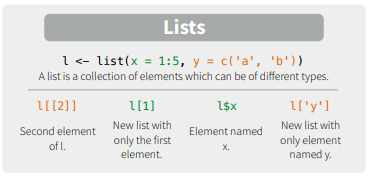
\includegraphics{images/03/05.PNG}

\begin{Shaded}
\begin{Highlighting}[]
\CommentTok{\#\# list}
\NormalTok{parent\_names <{-}}\StringTok{ }\KeywordTok{c}\NormalTok{(}\StringTok{"Fred"}\NormalTok{, }\StringTok{"Mary"}\NormalTok{)}
\NormalTok{number\_of\_children <{-}}\StringTok{ }\DecValTok{2}
\NormalTok{child\_ages <{-}}\StringTok{ }\KeywordTok{c}\NormalTok{(}\DecValTok{4}\NormalTok{, }\DecValTok{7}\NormalTok{, }\DecValTok{9}\NormalTok{)}
\KeywordTok{data.frame}\NormalTok{(parent\_names, number\_of\_children, child\_ages)}
\NormalTok{lst <{-}}\StringTok{ }\KeywordTok{list}\NormalTok{(parent\_names, number\_of\_children, child\_ages)}
\NormalTok{lst[}\DecValTok{1}\NormalTok{]}
\NormalTok{lst[[}\DecValTok{1}\NormalTok{]]}
\KeywordTok{class}\NormalTok{(lst[}\DecValTok{1}\NormalTok{])}
\KeywordTok{class}\NormalTok{(lst[[}\DecValTok{1}\NormalTok{]])}
\NormalTok{lst[[}\DecValTok{1}\NormalTok{]][}\DecValTok{1}\NormalTok{]}
\NormalTok{lst[[}\DecValTok{1}\NormalTok{]][}\KeywordTok{c}\NormalTok{(}\DecValTok{1}\NormalTok{,}\DecValTok{2}\NormalTok{)]}
\end{Highlighting}
\end{Shaded}

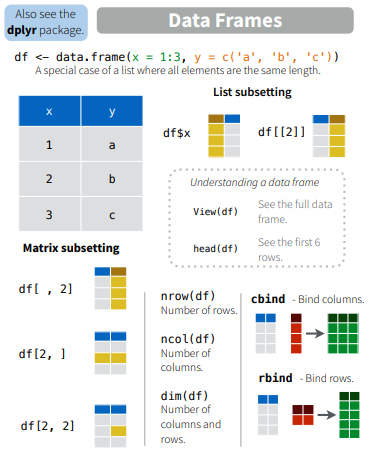
\includegraphics{images/03/06.PNG}

\hypertarget{missing-values}{%
\section{Missing values}\label{missing-values}}

특정 값이 ``Not available'' 이거나 ``Missing value'' 일 경우 벡터의 해당 원소 자리에 데이터의 이상을 알리기 위해 \texttt{NA}를 사용합니다. 따라서 일반적인 연산에서 \texttt{NA}가 포함되어 있는 경우 데이터의 불완전성을 알리기 위해 연산의 결과는 \texttt{NA}가 됩니다. \texttt{is.na()} 함수는 해당 변수에 \texttt{NA} 값이 있는지를 검사해주는 함수이며 R에는 이 외에도 다음과 같은 특수 값들이 사용되고 있습니다.

\begin{itemize}
\tightlist
\item
  NA: Not available, The value is missing
\item
  NULL: a reserved value
\item
  NaN: Not a number (0/0)
\item
  Inf: (1/0)
\end{itemize}

\begin{Shaded}
\begin{Highlighting}[]
\NormalTok{hip\_cost <{-}}\StringTok{ }\KeywordTok{c}\NormalTok{(}\DecValTok{10500}\NormalTok{, }\DecValTok{45000}\NormalTok{, }\DecValTok{74100}\NormalTok{, }\OtherTok{NA}\NormalTok{, }\DecValTok{83500}\NormalTok{)}
\KeywordTok{sum}\NormalTok{(hip\_cost)}
\KeywordTok{sum}\NormalTok{(hip\_cost, }\DataTypeTok{na.rm=}\OtherTok{TRUE}\NormalTok{)}
\NormalTok{?sum}
\end{Highlighting}
\end{Shaded}

\hypertarget{useful-functions-i}{%
\section{Useful functions I}\label{useful-functions-i}}

다음은 벡터형 변수와 같이 쓰이는 유용한 함수들입니다.

\begin{Shaded}
\begin{Highlighting}[]
\NormalTok{z <{-}}\StringTok{ }\KeywordTok{sample}\NormalTok{(}\DecValTok{1}\OperatorTok{:}\DecValTok{10}\NormalTok{, }\DecValTok{100}\NormalTok{, T)}
\KeywordTok{head}\NormalTok{(z)}
\KeywordTok{sort}\NormalTok{(z)}
\KeywordTok{order}\NormalTok{(z)}
\KeywordTok{table}\NormalTok{(z)}
\NormalTok{p <{-}}\StringTok{ }\NormalTok{z}\OperatorTok{/}\KeywordTok{sum}\NormalTok{(z)}
\KeywordTok{round}\NormalTok{(p, }\DataTypeTok{digits=}\DecValTok{1}\NormalTok{)}
\NormalTok{digits <{-}}\StringTok{ }\KeywordTok{as.character}\NormalTok{(z)}
\NormalTok{n <{-}}\StringTok{ }\KeywordTok{as.numeric}\NormalTok{(digits)}
\NormalTok{d <{-}}\StringTok{ }\KeywordTok{as.integer}\NormalTok{(digits)}
\end{Highlighting}
\end{Shaded}

\hypertarget{exercise-3-5}{%
\subsection{Exercise 3-5}\label{exercise-3-5}}

\begin{itemize}
\tightlist
\item
  score 라는 변수에 1부터 100까지 중 랜덤하게 선택된 20개의 수로 10 x 2 matrix를 만드시오
\item
  score의 row 이름을 문자형으로 Name1, Name2, \ldots, Name10으로 지정하시오 (\texttt{paste()}변수 사용)
\item
  score의 column 이름을 문자형으로 math와 eng로 지정하시오
\item
  이 matrix의 첫번째 컬럼과 두 번째 컬럼의 수를 각각 더한 후 total\_score라는 변수에 저장 하시오
\item
  total\_score 오름차순 순서를 나타내는 인덱스 (\texttt{order()}함수 사용)를 o라는 변수에 저장 하시오
\item
  score를 o순서로 재 배치 하고 score\_ordered 변수에 저장 하시오
\end{itemize}

\begin{center}\rule{0.5\linewidth}{0.5pt}\end{center}

이 저작물은 크리에이티브 커먼즈 저작자표시-비영리-변경금지 4.0 국제 라이선스에 따라 이용할 수 있습니다.

\end{document}
